\section{Simulations}\label{sec:simulation}
We utilized MATLAB simulations with Simulink to validate the efficiency of CBFs in various robotic systems and to compare the performance of model-free techniques with classical ones. We made an effort to maintain as many simulation parameters as possible to be consistent throughout the process. The structure of all the control blocks for the model-free method follows the basic scheme reported in Figure~\ref{fig:simulink}. Here, we have always implemented a model-independent controller to track the safe velocity generated utilizing knowledge from a reduced-order model, as opposed to the real one representing the robotic system. The classical method does not utilize a safe velocity
\begin{figure}[H]
    \centering
    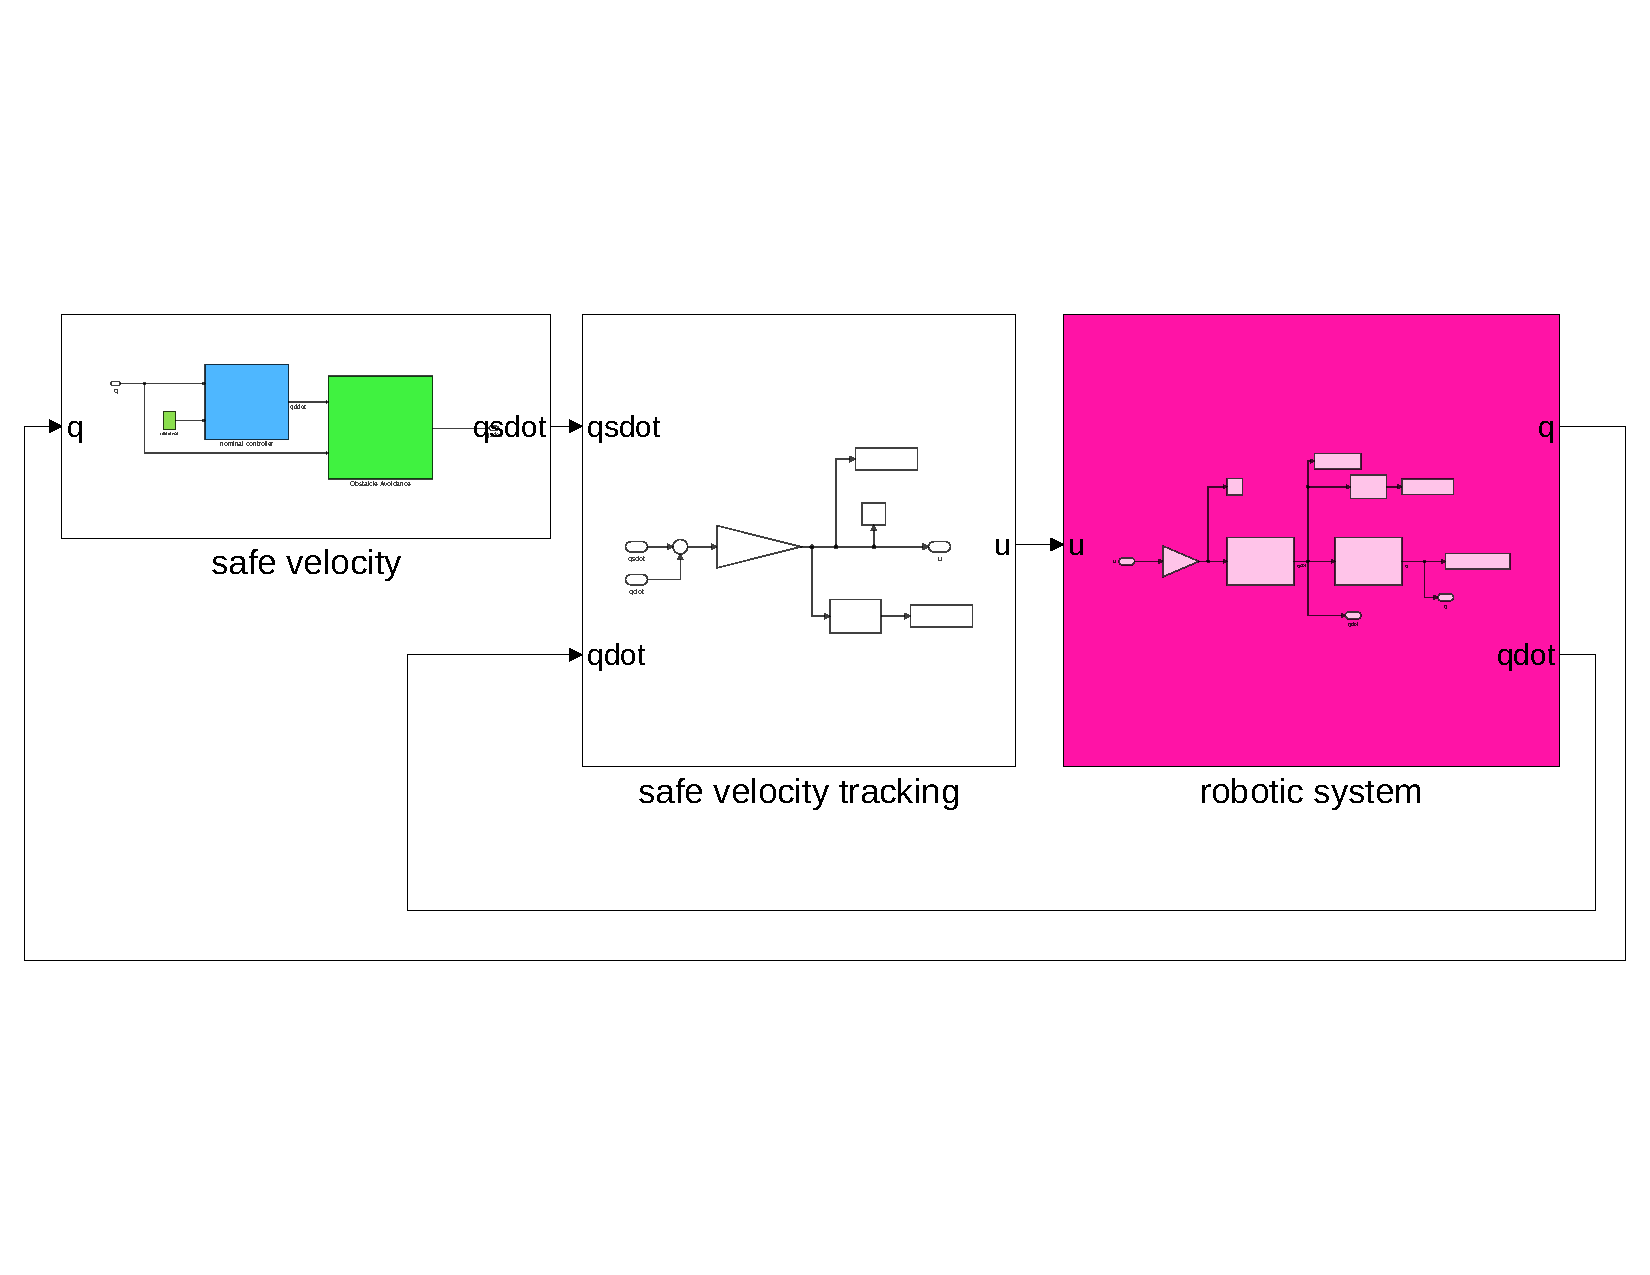
\includegraphics[width=11cm]{../figures/schema.pdf}
    \caption{Control block structure of our model-free approach implementation. The robotic system \eqref{eq:dynamic model} outputs the pose and velocities, only the former takes a role in the safe velocity generation while the latter are used to track it.}
    \label{fig:simulink}
\end{figure}
\noindent
tracker, as the input is directly provided to the robot. This approach does not make use of an approximation of the dynamics and takes into account both the pose and velocity in generating the safe input.
%Let us define the set $\mathcal{O}=\{\qv_{\mathcal{O}_i}\in\mathbb{R}^n,i=1,..,m\}$ and associate to each obstacle $\mathcal{O}_i$, the corresponding control barrier function $h_i(\qv)$.

\subsection{Point robot}
For the first simulations, as the simplest instance of \eqref{eq:dynamic model}, let us consider a point robot, which dynamics can be modeled by: 
\begin{equation}\label{eq:pr dyn}
    \Mm\ddot{\qv} = \Bm\uv,
\end{equation}
where $\qv \in \mathbb{R}^2$ represents the planar position of the robot, $\uv \in \mathbb{R}^2$, $\Bm=\boldsymbol{I}_{2}$ and $\Mm = \mbox{diag}\left\{m, m\right\}$ in this scenario.
%A possible unsafe tracking controller which allows the robot to go from $\qv_{start}$ to $\qv_{goal}$ without taking into account the obstacles is given by :
We want to solve the problem of guiding the system from an initial configuration $\qv_{start}$ to a final one $\qv_{goal}$ while avoiding circular obstacles thanks to the CBF, therefore remaining in the safe region.
%, firstly,  in a model-free fashion and, then, in the classical full-model based approach.
% We work with multiple obstacles with  different dimensions.
% The first simulation 
% \textbf{Model-free Approach}:
\subsubsection{Model-free}
A solution that allows navigating from $\qv_{start}$ to $\qv_{goal}$ without taking into account the obstacles consists in realizing the nominal velocity   
\begin{equation}
    \dot{\qv}_{nom}=-K_P(\qv - \qv_{goal}),\,K_P\in\mathbb{R}_{>0}.
\end{equation}
We can modify it, in a minimally invasive fashion attaining $\dqv_{safe}$ by solving the optimization problem \eqref{eq:optprob} using as CBF
\begin{equation}\label{eq:cbfsim1}
h_i(\qv)=d_{i}-R_{\mathcal{O}_i}
\end{equation}
 where $R_{\mathcal{O}_i}$ is the radius of the obstacle centered at $\qv_{\mathcal{O}_i}$ and $d_{i} = \lVert \qv-\qv_{\mathcal{O}_i} \rVert$.
% with gradient $\nabla h(\qv) = (\qv-\qv_O)/d = \nv_0$. 
%So we modify $\dot{\qv}_{nom}$ in a minimally invasive fashion by solving the optimization problem \eqref{eq:optprob} attaining the safe velocity $\dot{\qv}_{safe}$.
When $h_i(\qv)$ is positive it means that there is no collision with $\mathcal{O}_i$.
In Simulation 1 to track $\dqv_{safe}$ we used controller \eqref{eq:mf controller}. Here, the robot starts at rest from $\qv_{start}=(0,0)^T$ and the goal is $\qv_{goal}=(4,-1)^T$, while the obstacles positions are $\qv_{\mathcal{O}_1}=(1.5,0)^T$, $\qv_{\mathcal{O}_2}=(3,-1.5)^T$ with common radius $R=0.75$. Setting the gains $K_P = 0.2,~\Km_D=\boldsymbol{I}_{2x2}$, $m=1$~[Kg] and considering at each time the closest object for the CBF \eqref{eq:cbfsim1}, we have been able to reproduce exactly the simulation proposed in \cite{mfcbf} varying $\alpha$, as shown in Figure~\ref{fig:sim1map}.
Note that, even though $\alpha=0.5 < \lambda = 1$, the CBF becomes negative because the robot is passing through the obstacle $\mathcal{O}_2$. This is an interesting result since it highlights how, when the exponential tracking of the safe velocity is not guaranteed Figure~\ref{fig:sim1v}, Theorem \ref{th:alpha limit} does not hold, meaning that safety is lost. 
For this reason, in Simulation 2 we decided to guarantee ISSf with respect to the full model disturbance $\dv = -\Mm\ddot{\qv}_{safe}$. We have estimated $\ddqv_{safe}$ through Simulink with a backward derivative block after $\dqv_{safe}$ used to solve the same problem. Setting $\alpha=0.99$ and without changing the other Simulation 1 parameters, resulted in $||\dv||_\infty = 0.5$, obtaining $\gamma = 0.3571$. In order to limit the values for $\gamma$ the best approach is to set $\alpha$ as large as possible. Intuitively, this method can be understood as ensuring safety with respect to a reduced set, which accurately reflects the true size of the safe set by incorporating the uncertainty from the disturbance $\dv$. This is implemented as an additional clearance equal to $\gamma$ that prevents the robot from hitting the obstacles even in the case of tracking errors. 
Therefore even if the CBF is lower than the $\gamma$ bound in certain instants, meaning that the considered CBF is negative, safety is still maintained since collisions with the obstacles are avoided.
This additional clearance has resulted in better performances as shown in Figures \ref{fig:sim2map}--\ref{fig:sim2in}.
\subsubsection{Model-based CBF}
In Simulation 3, in order to approach the same problem directly through the full dynamic model, it is not possible to use CBF \eqref{eq:cbfsim1} since it misses the \textit{relative-degree} one condition with respect to \eqref{eq:pr dyn}. 
Therefore, we augmented it by adding a velocity term that lets the new $h$ decrease if the robot is moving towards the obstacle and increase on the contrary, as proposed in \cite{vendittelli}
\begin{equation}\label{eq:difmcbf}
    h(\qv,\dqv)=||\qv-\qv_\mathcal{O}||^2+\mu(\qv-\qv_\mathcal{O})^T\dqv,
\end{equation}
with $\mu$ a positive constant, set to $0.8$ in this simulation. We used this in the optimization problem to correct the nominal input generated with:
\begin{equation}
\uv_{nom}=-K_P(\qv - \qv_{goal})-K_D \dqv,
\end{equation}
using $K_P = 0.2, K_D = 1$, the same gains of Simulation 1 and $\alpha = 1$.
As depicted in Figure~\ref{fig:sim3map}, it is clear that access to the dynamic system enables the robot to fully utilize the safe region without any concerns regarding uncertainties in the model.
\begin{center}
\begin{figure}[H]
\begin{minipage}[b]{0.45\linewidth}
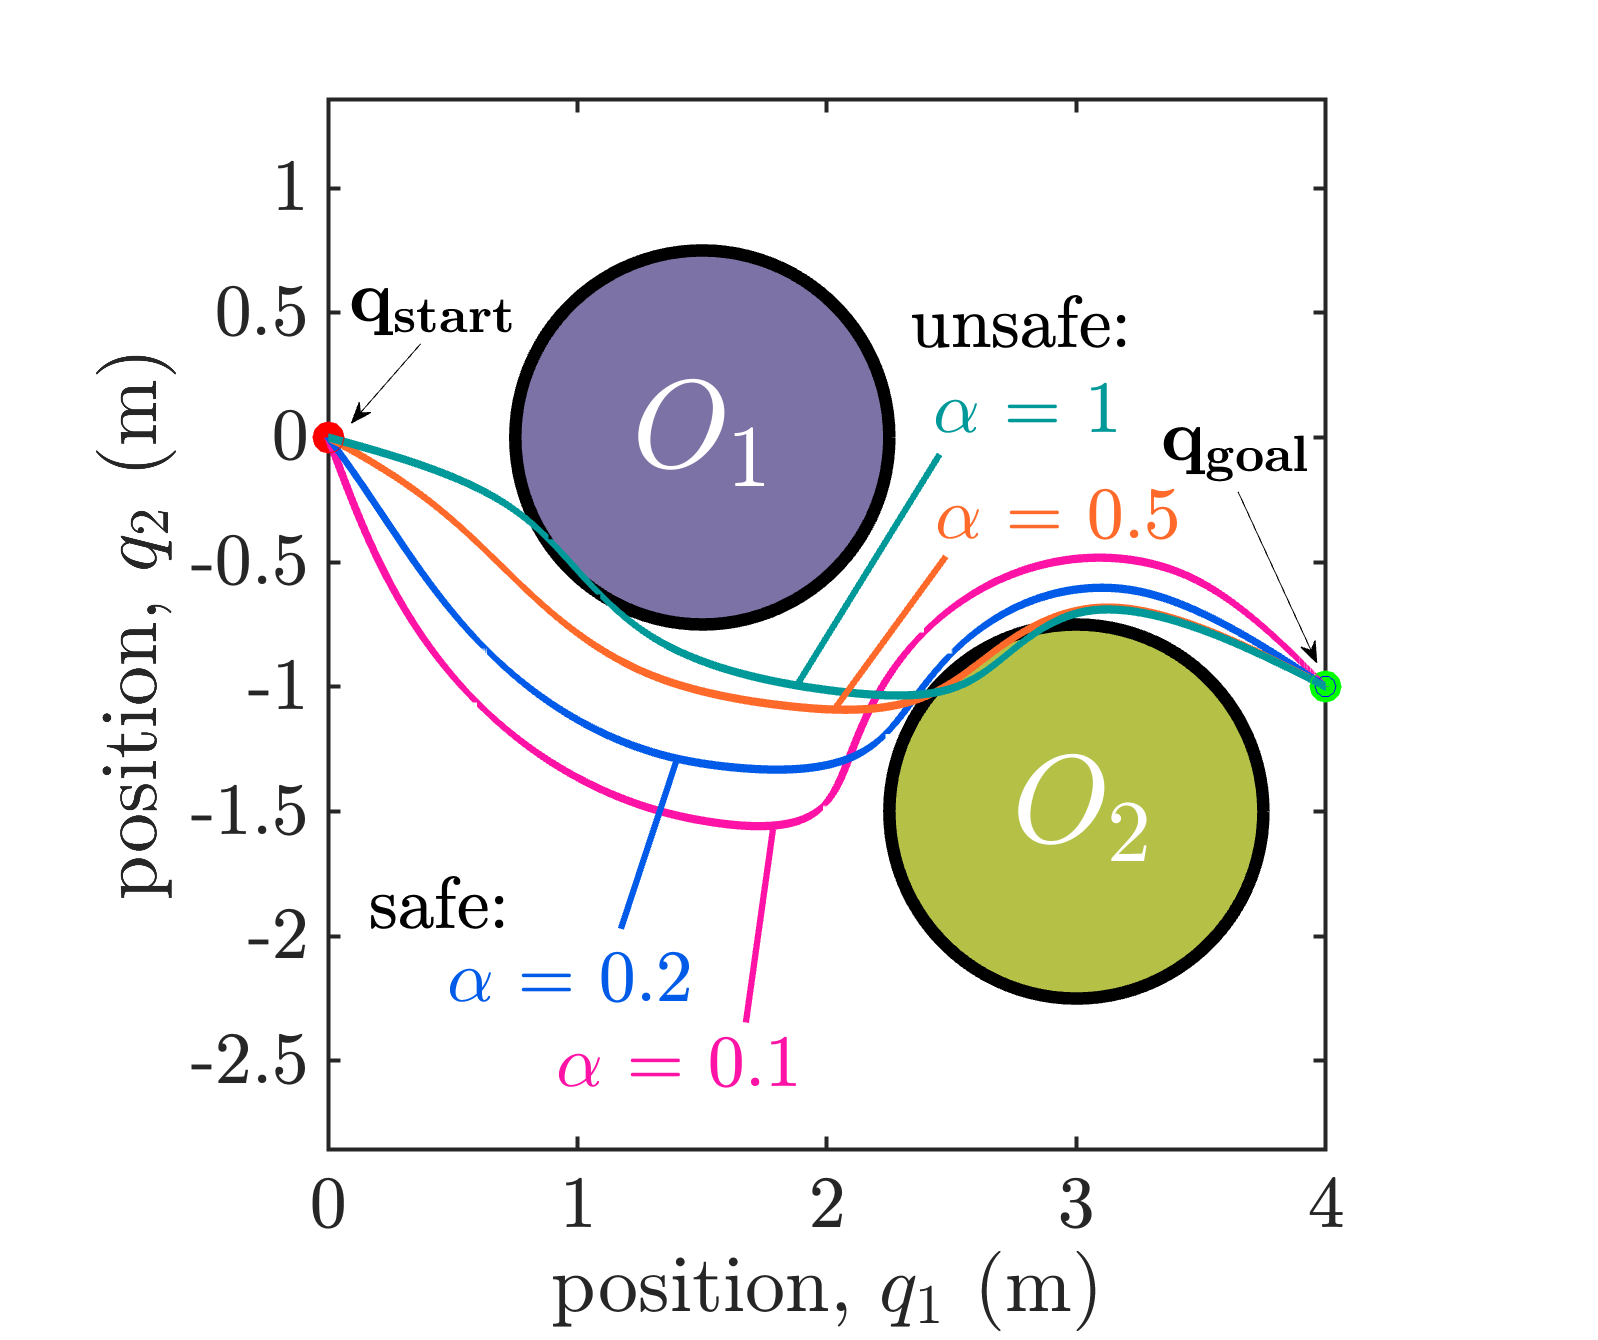
\includegraphics[scale=0.30,trim={1.7cm 0 0 0},clip]{figures/sim1map.pdf}
\caption{\label{fig:sim1map}Simulation 1: evolution of the state $\qv$ over the environment for the different values of parameter $\alpha$.}
\end{minipage}
\hfill
\begin{minipage}[b]{0.44\linewidth}
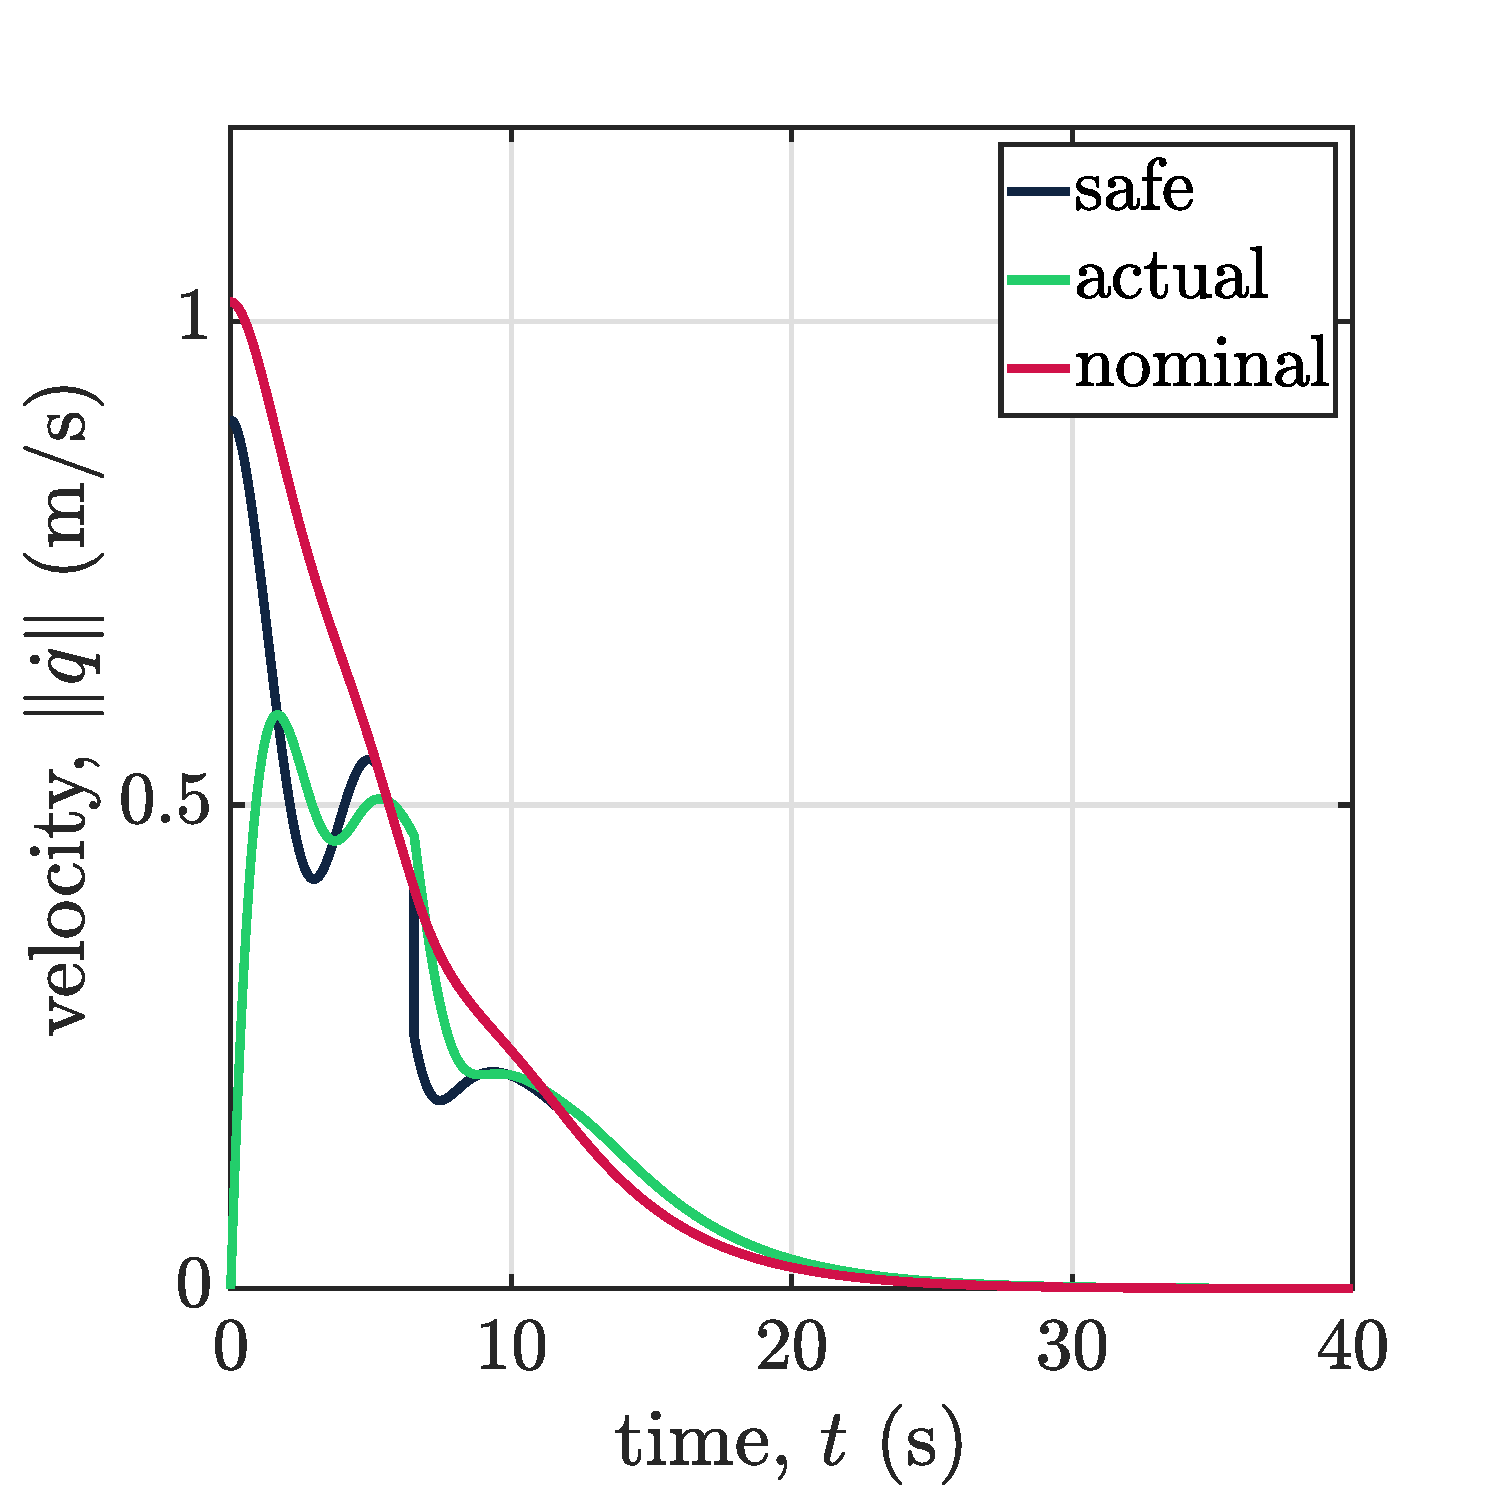
\includegraphics[scale=0.27]{figures/sim1vn.eps}
\caption{\label{fig:sim1v}Simulation 1: evolution of the velocity norms $|\dqv|$ for $ \alpha = 0.5$.\\~}
\end{minipage}
\end{figure}
\end{center}
\clearpage
%new fig
\begin{figure}[!ht]
    \begin{minipage}[b]{0.46\linewidth}
    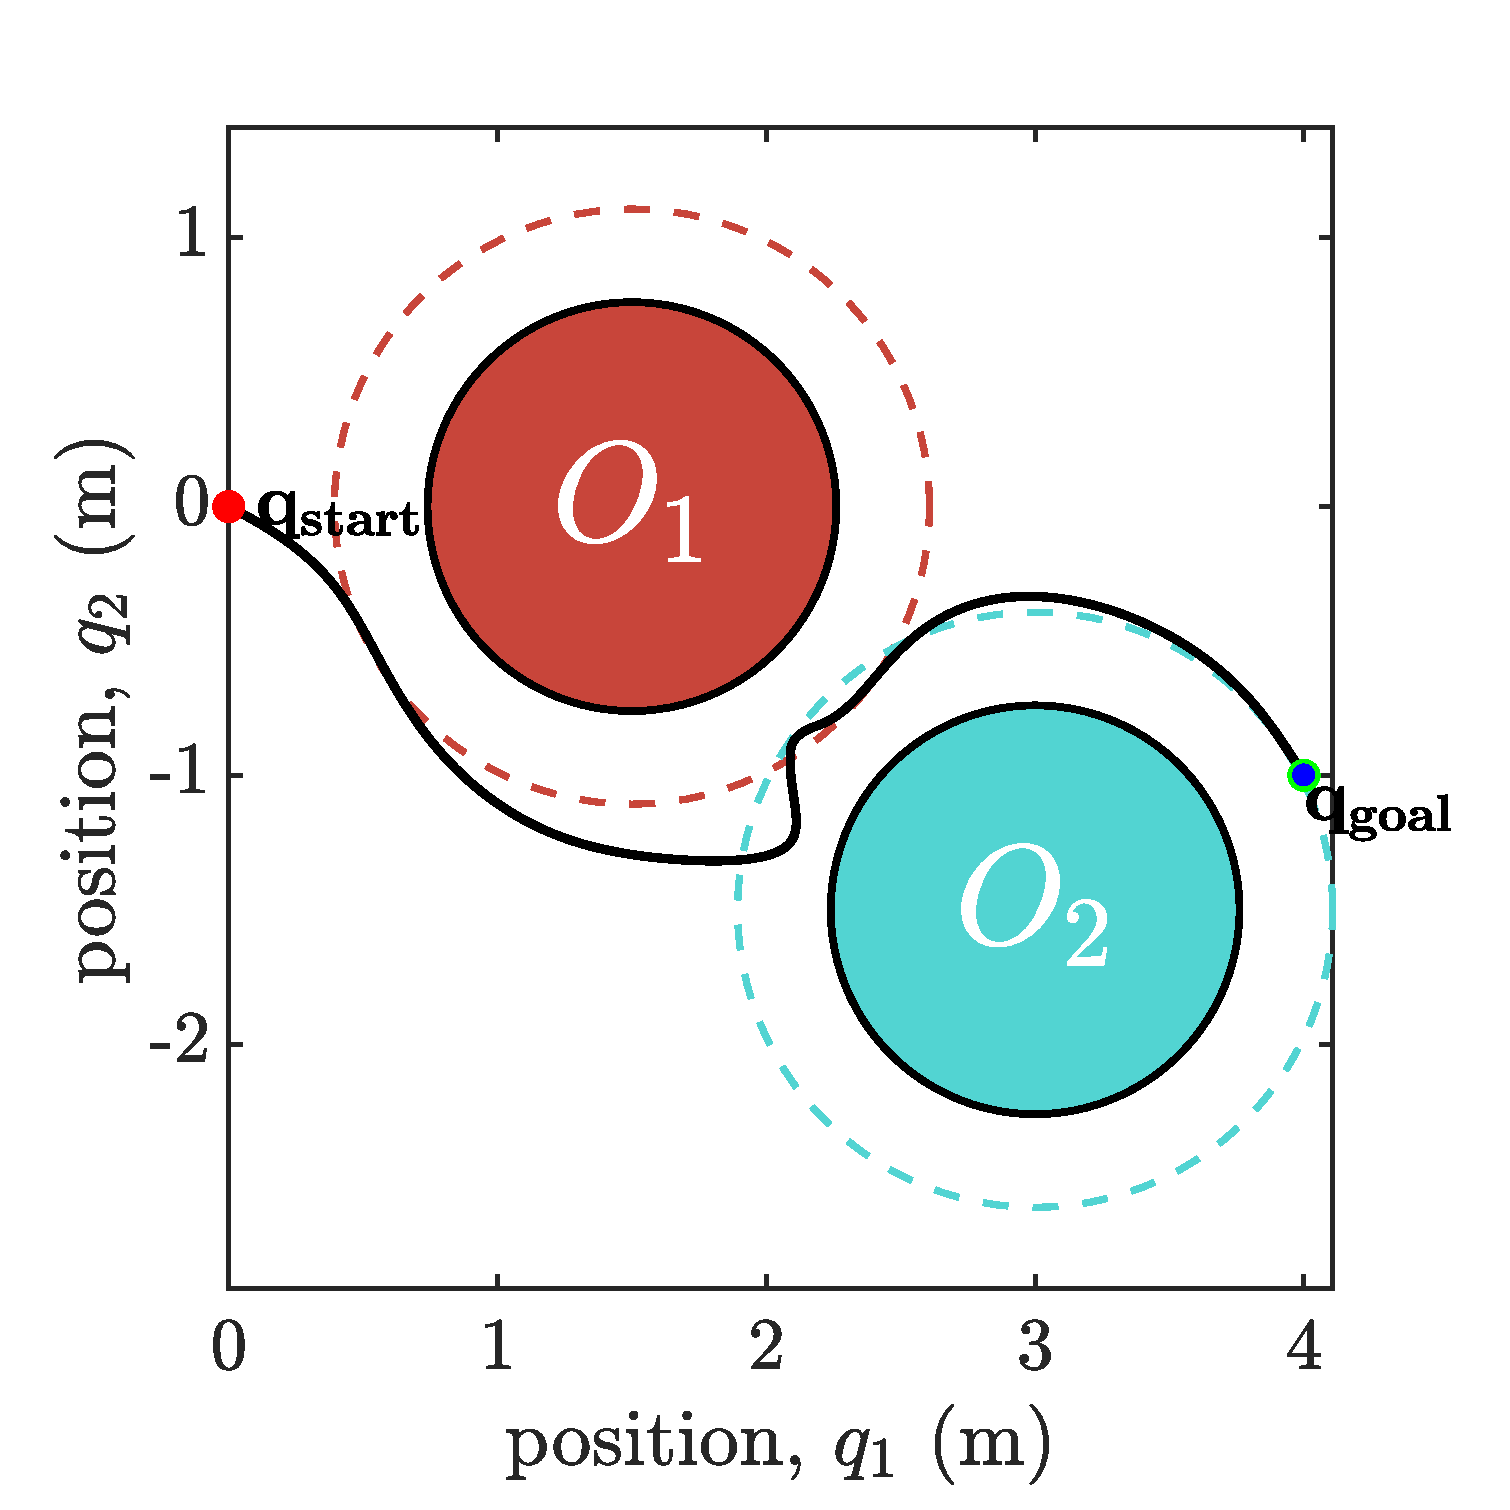
\includegraphics[width=\textwidth]{figures/sim2map.eps}
    \caption{\label{fig:sim2map}Sim. 2: evolution of the state $\qv$ over the environment.}
    \end{minipage}
    \hfill
    \begin{minipage}[b]{0.46\linewidth}
    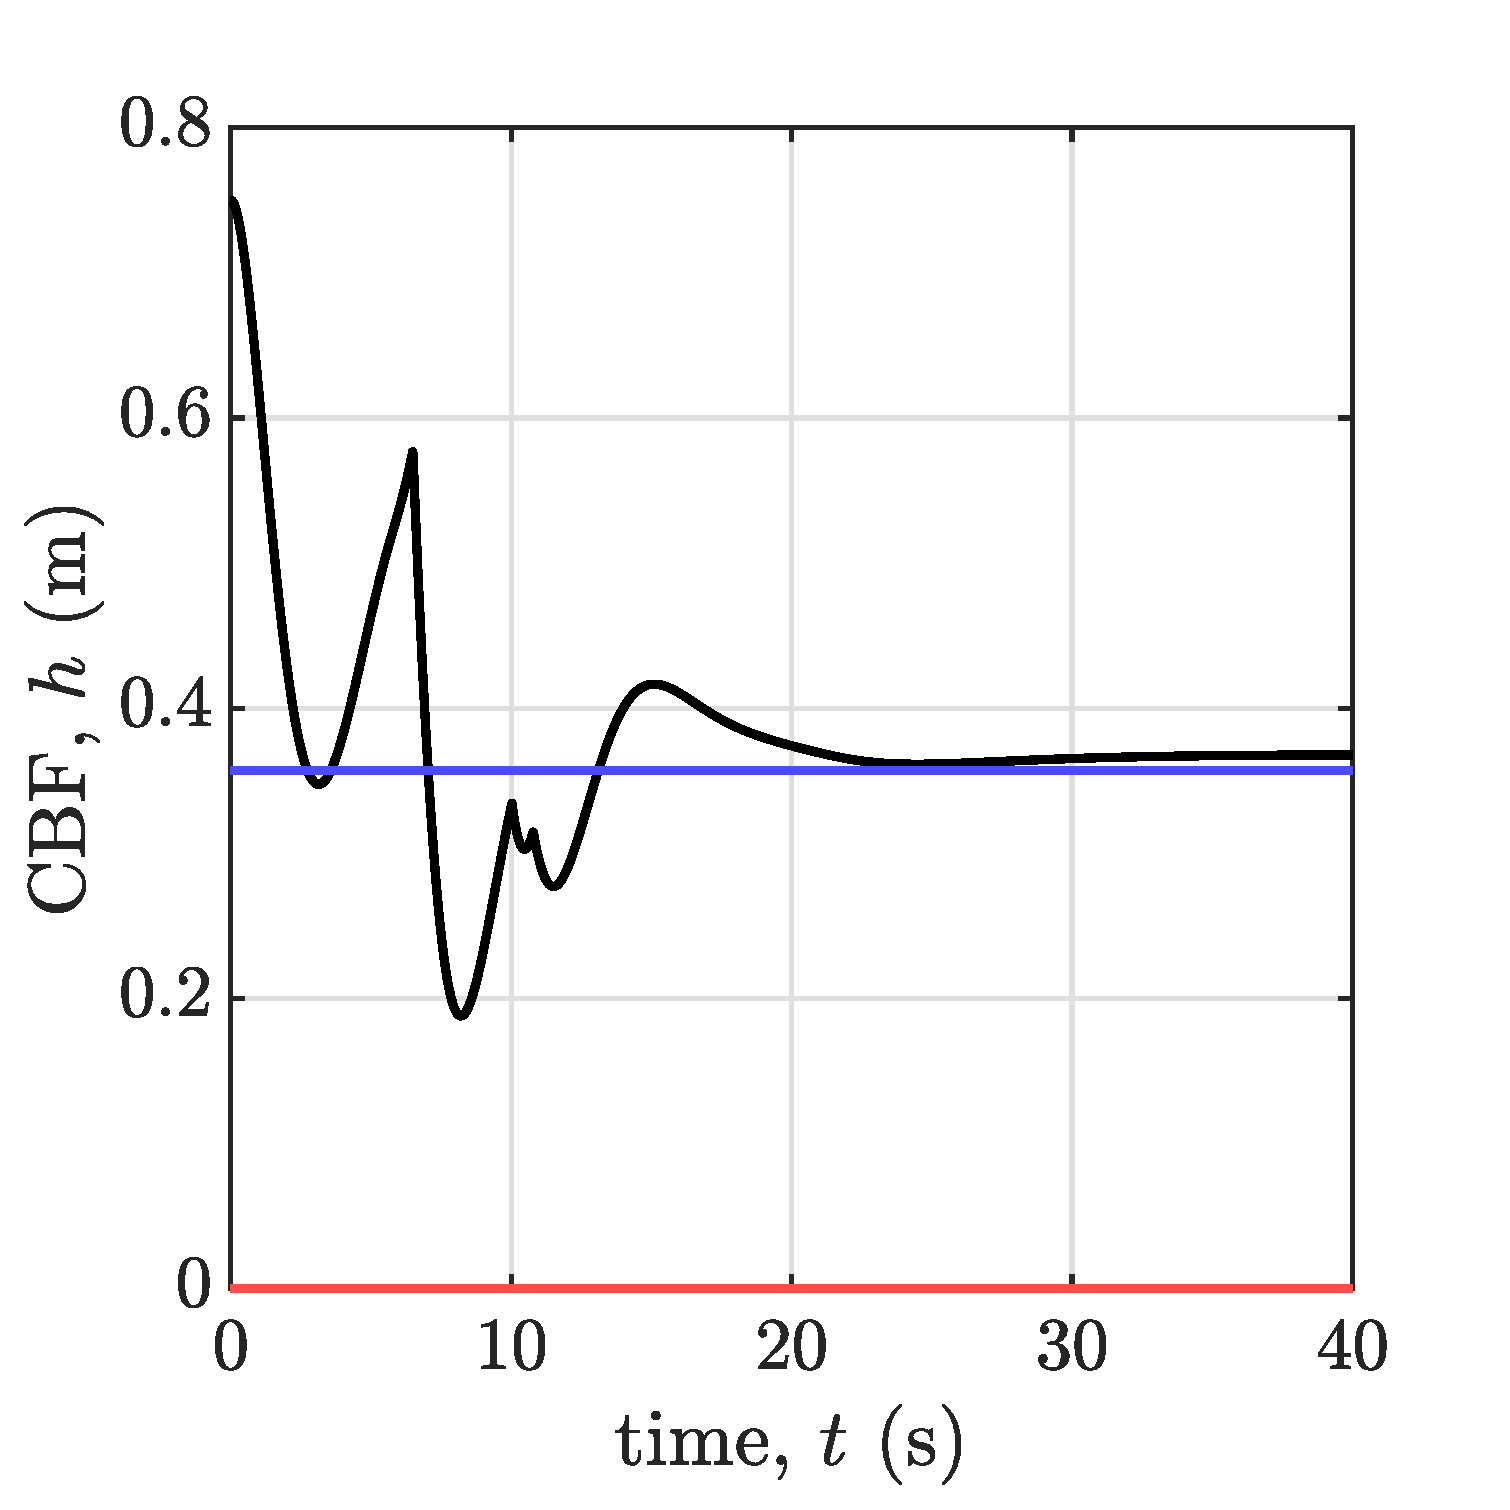
\includegraphics[width=\textwidth]{figures/sim2h.eps}
    \caption{\label{fig:sim2h}Sim 2: evolution of $h$ with $\gamma = 0.3571\,[\mathrm{m}$] (blue line).}
    \end{minipage}
    \begin{minipage}[t]{.45\textwidth}
        \centering
        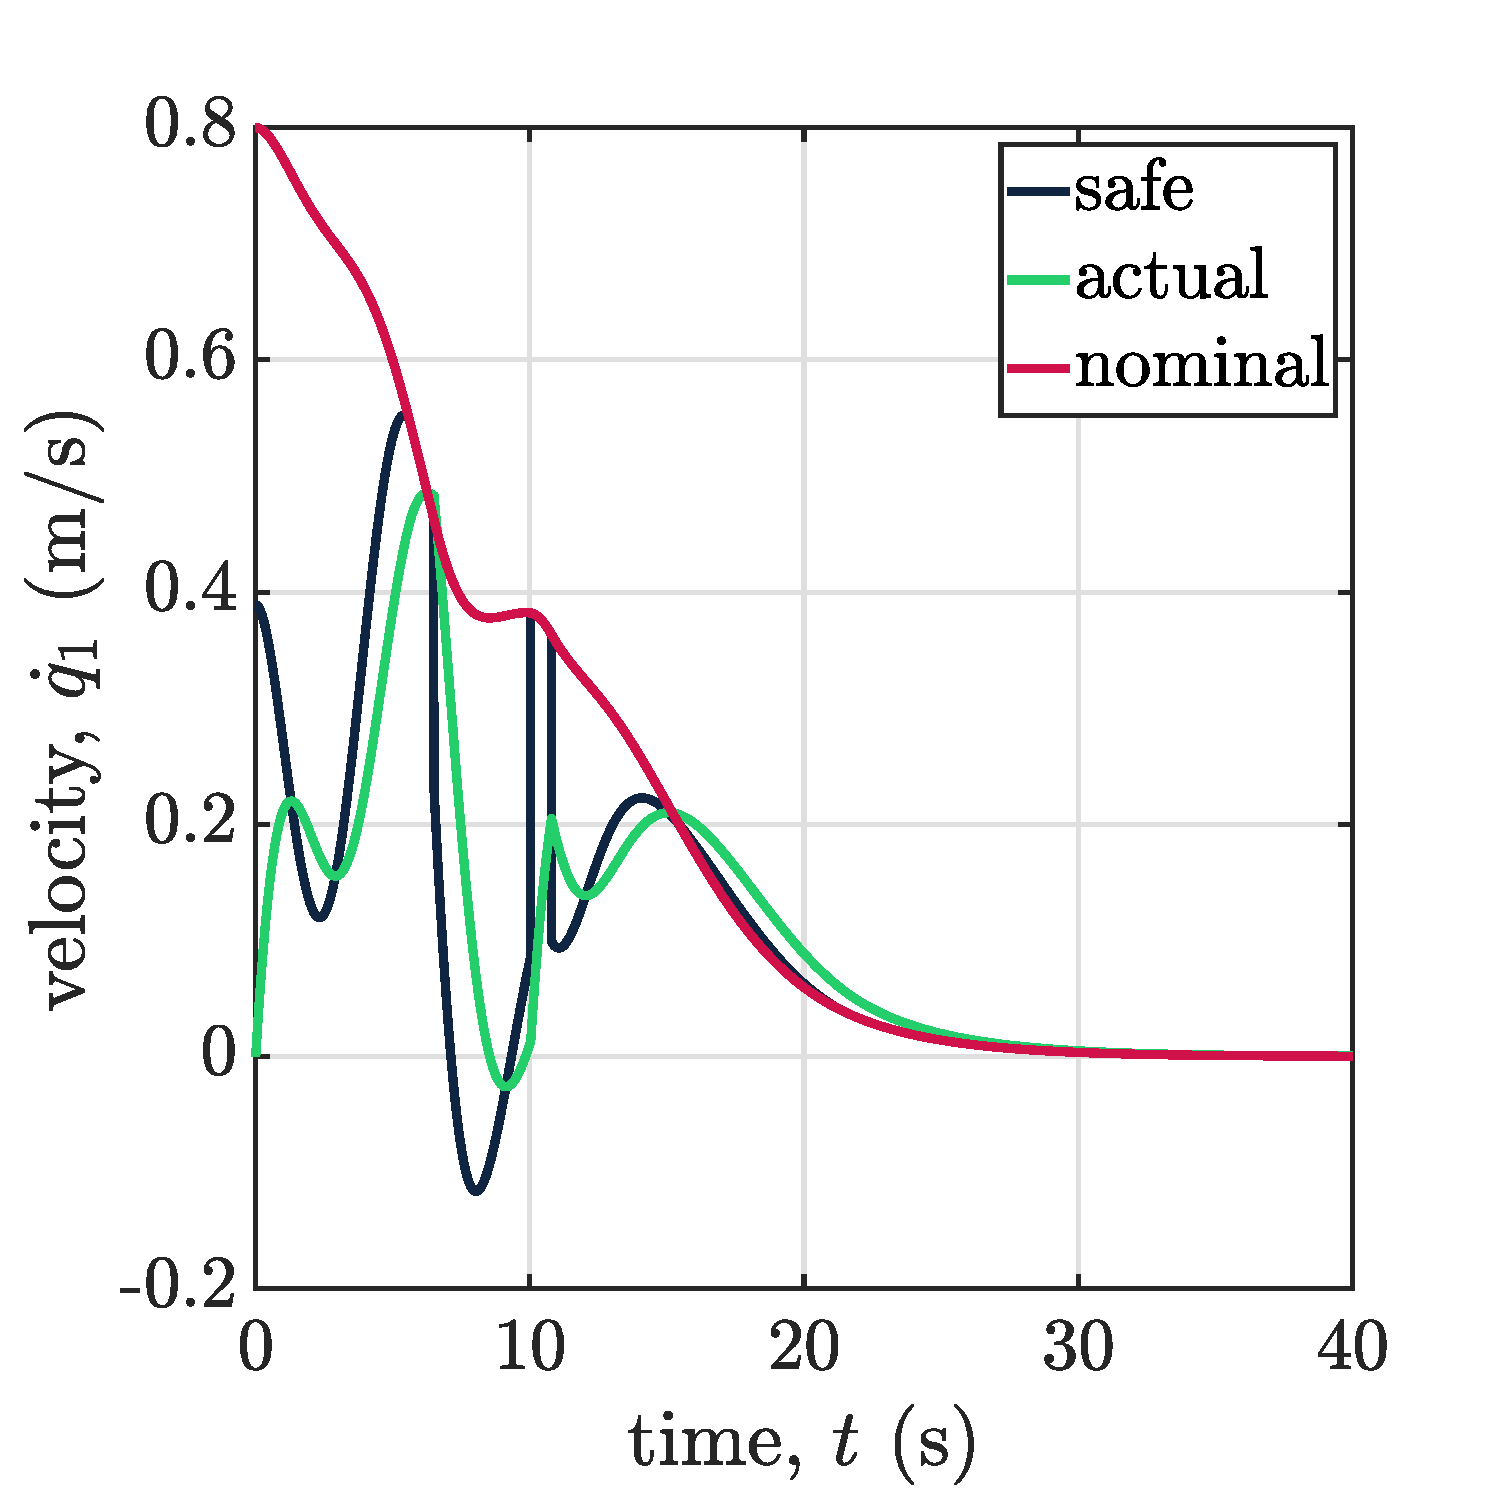
\includegraphics[width=\textwidth]{figures/sim2vel1.eps}
    \end{minipage}
    \hfill
    \begin{minipage}[t]{.45\textwidth}
        \centering
        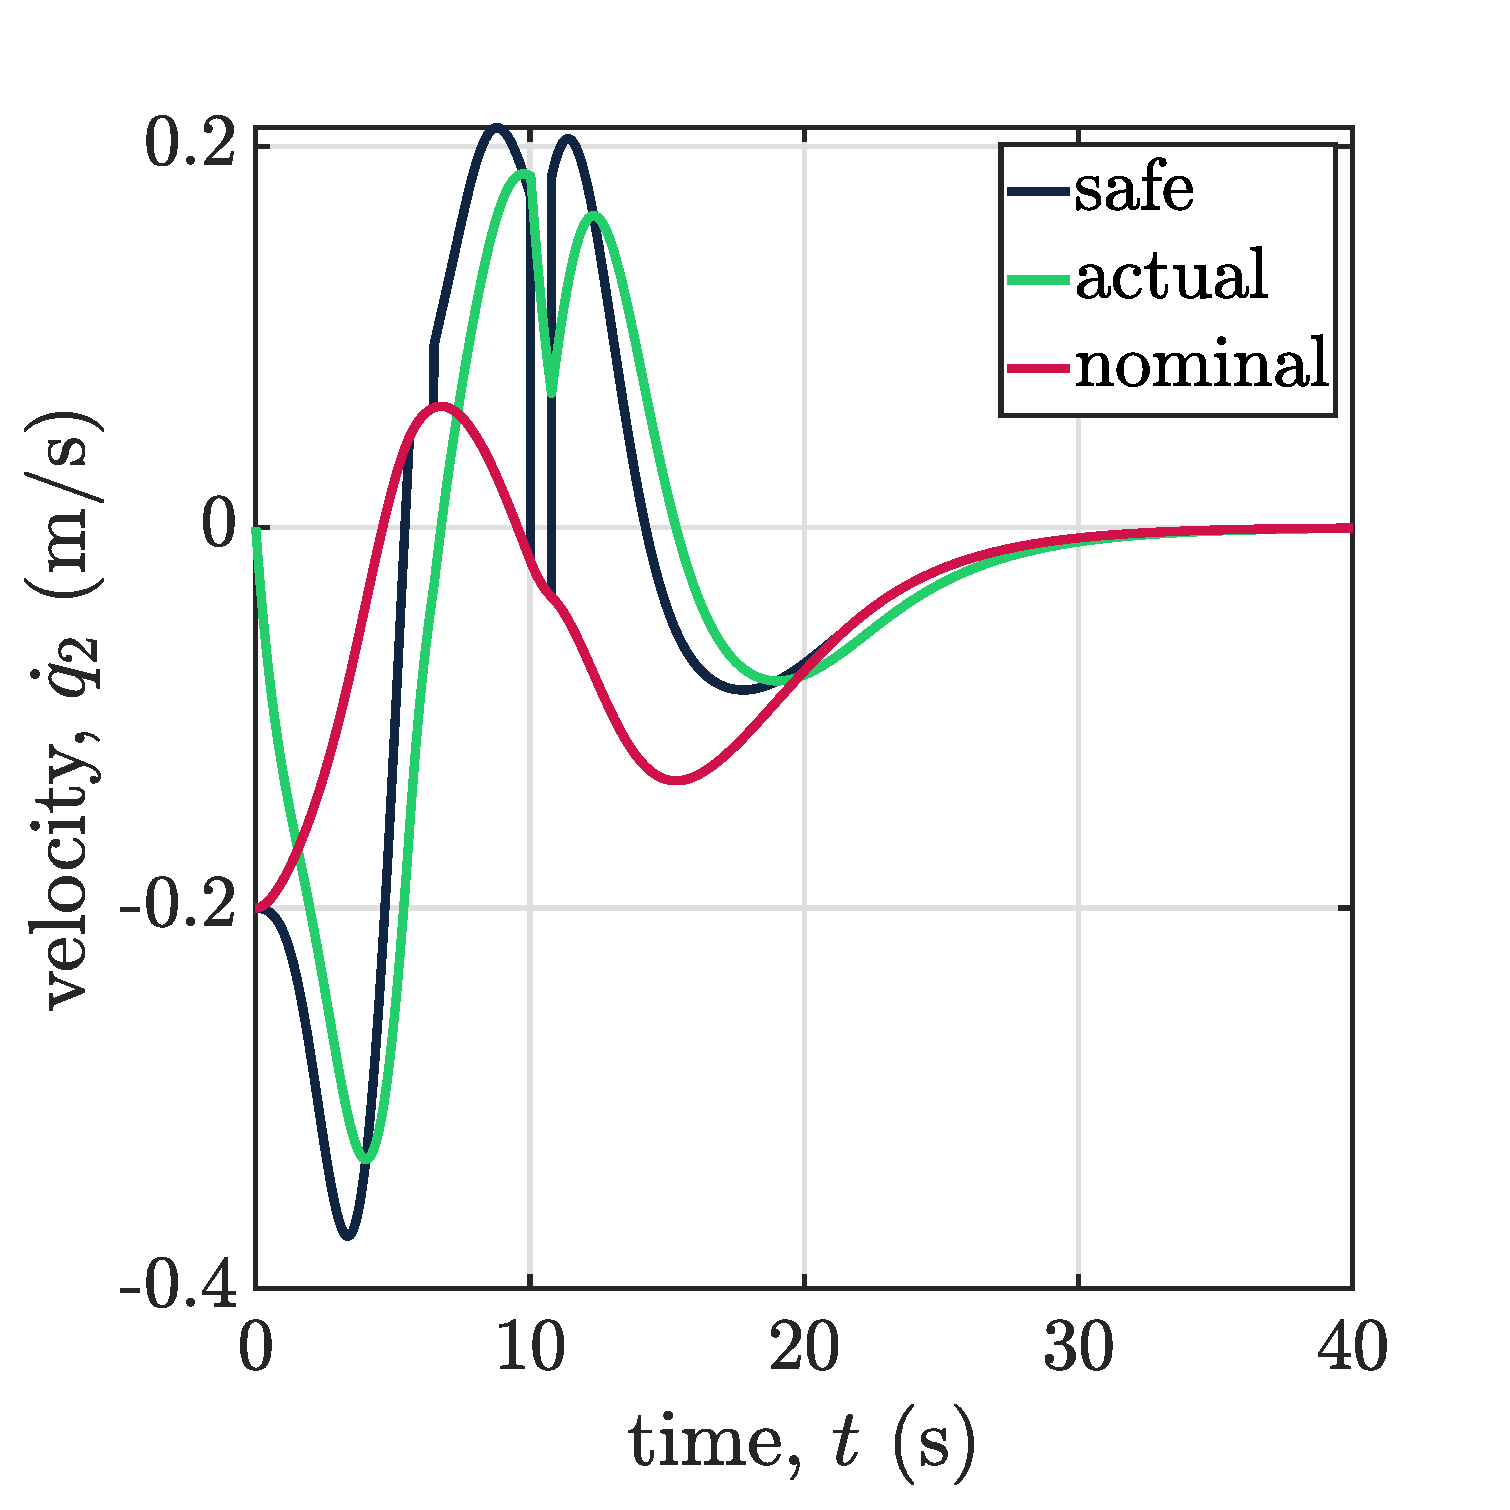
\includegraphics[width=\textwidth]{figures/sim2vel2.eps}
    \end{minipage}  
    \caption{\label{fig:sim2vel}Sim 2: Evolution of the velocity vector $\dqv$ components}
    \begin{minipage}[t]{.45\textwidth}
        \centering
        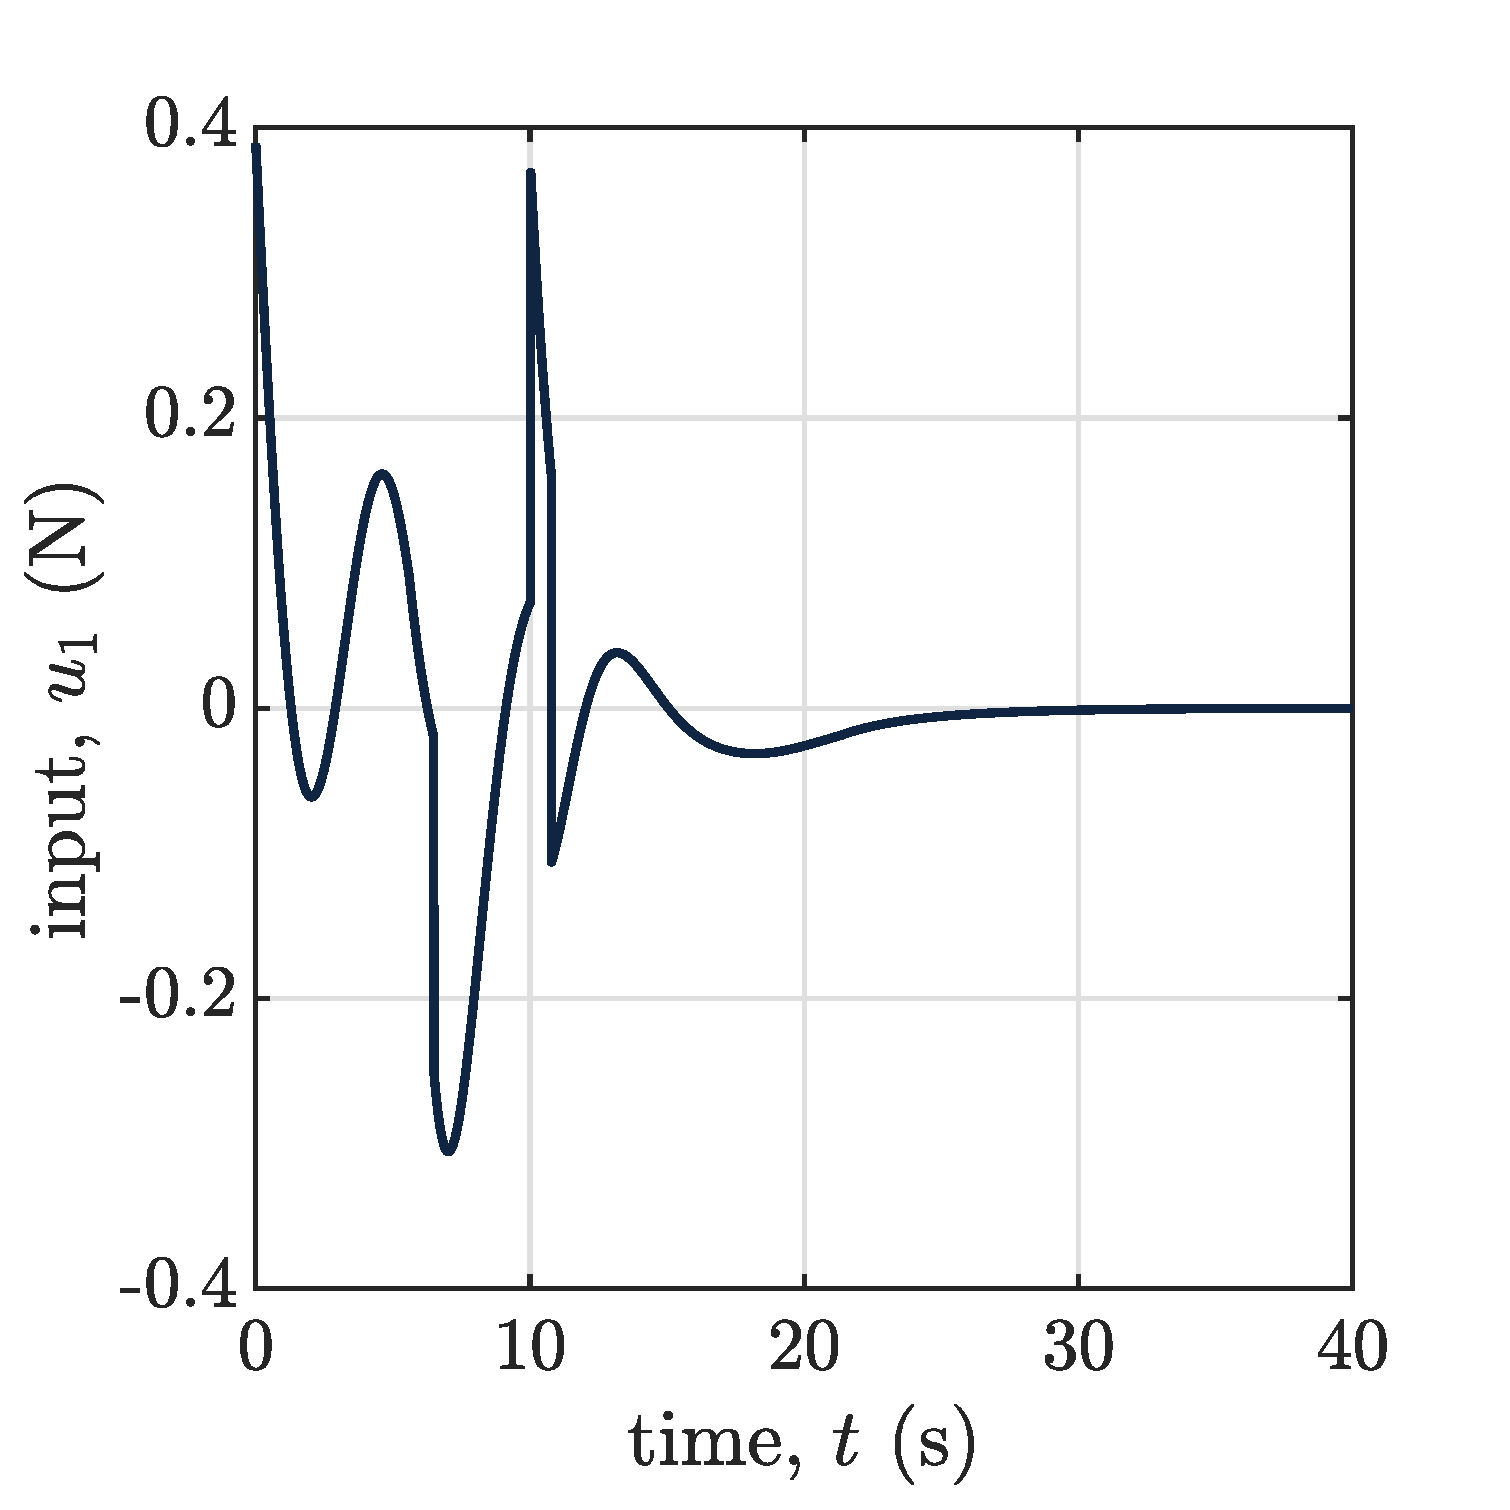
\includegraphics[width=\textwidth]{figures/sim2u1.eps}
    \end{minipage}
    \hfill
    \begin{minipage}[t]{.45\textwidth}
        \centering
        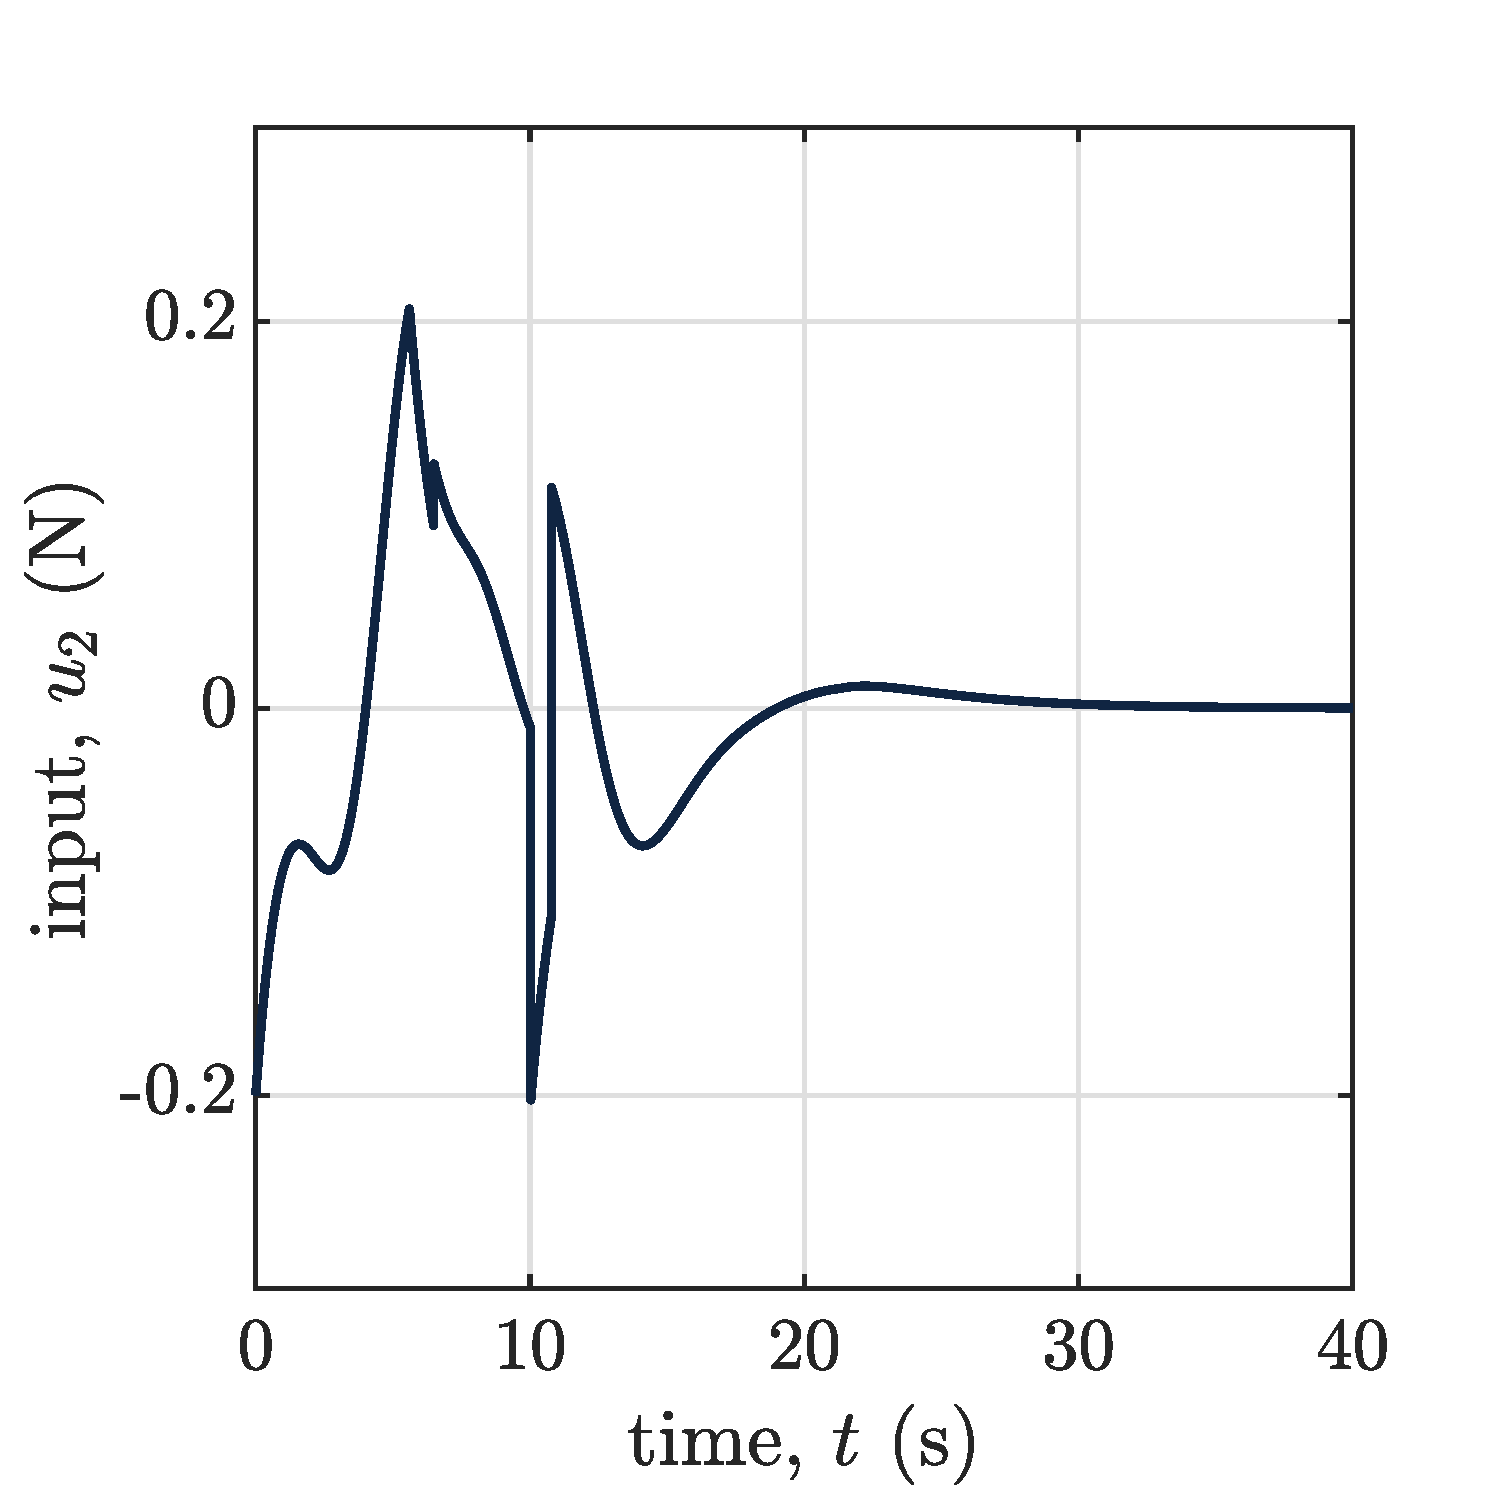
\includegraphics[width=\textwidth]{figures/sim2u2.eps}
    \end{minipage} 
    \caption{\label{fig:sim2in}Sim 2: Evolution of the input vector $\uv$ components}
\end{figure}
\clearpage
\newpage
% Simulation 3 
\begin{figure}[!ht]
    \begin{minipage}[b]{0.46\linewidth}
    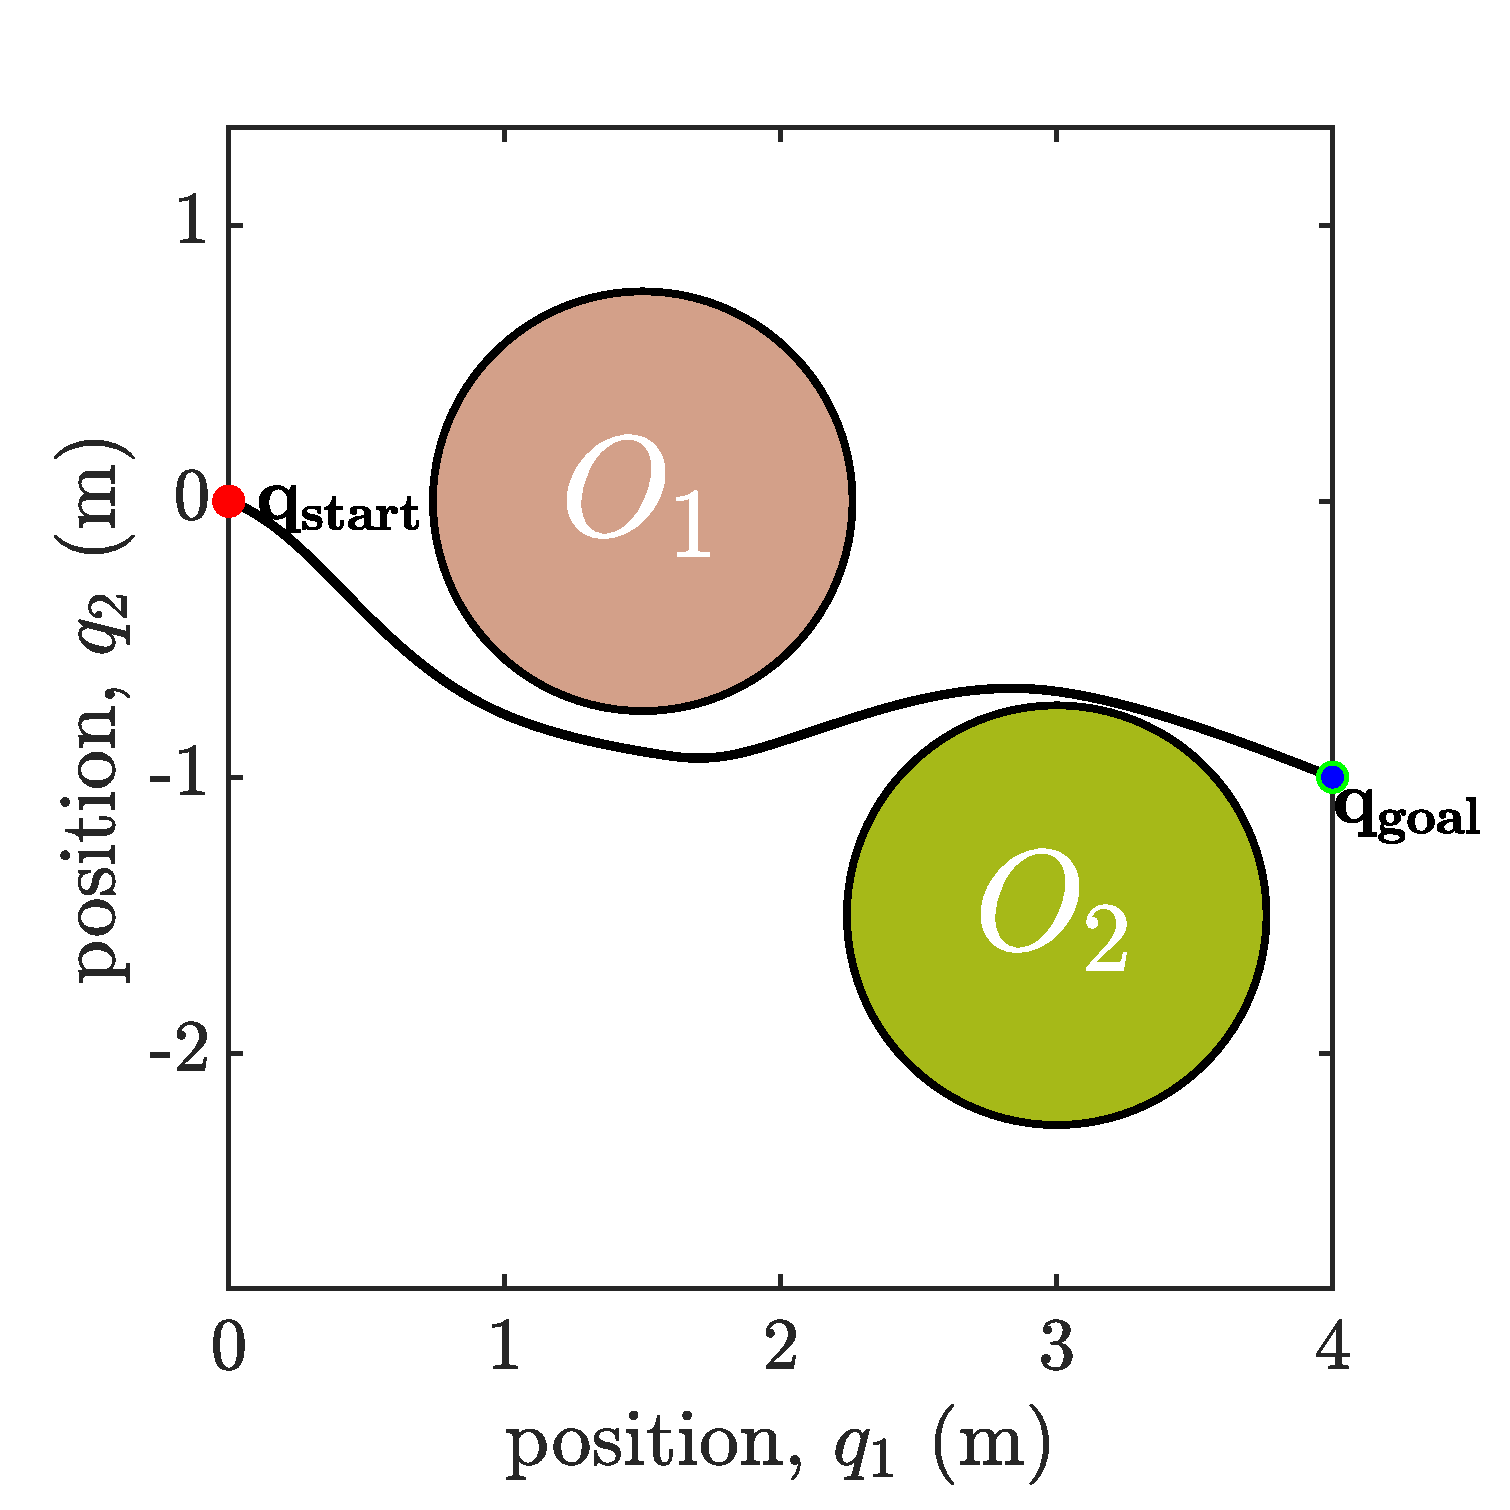
\includegraphics[width=\textwidth]{figures/sim3map.eps}
    \caption{\label{fig:sim3map}Sim. 3: evolution of the state $\qv$ over the environment.}
    \end{minipage}
    \hfill
    \begin{minipage}[b]{0.46\linewidth}
    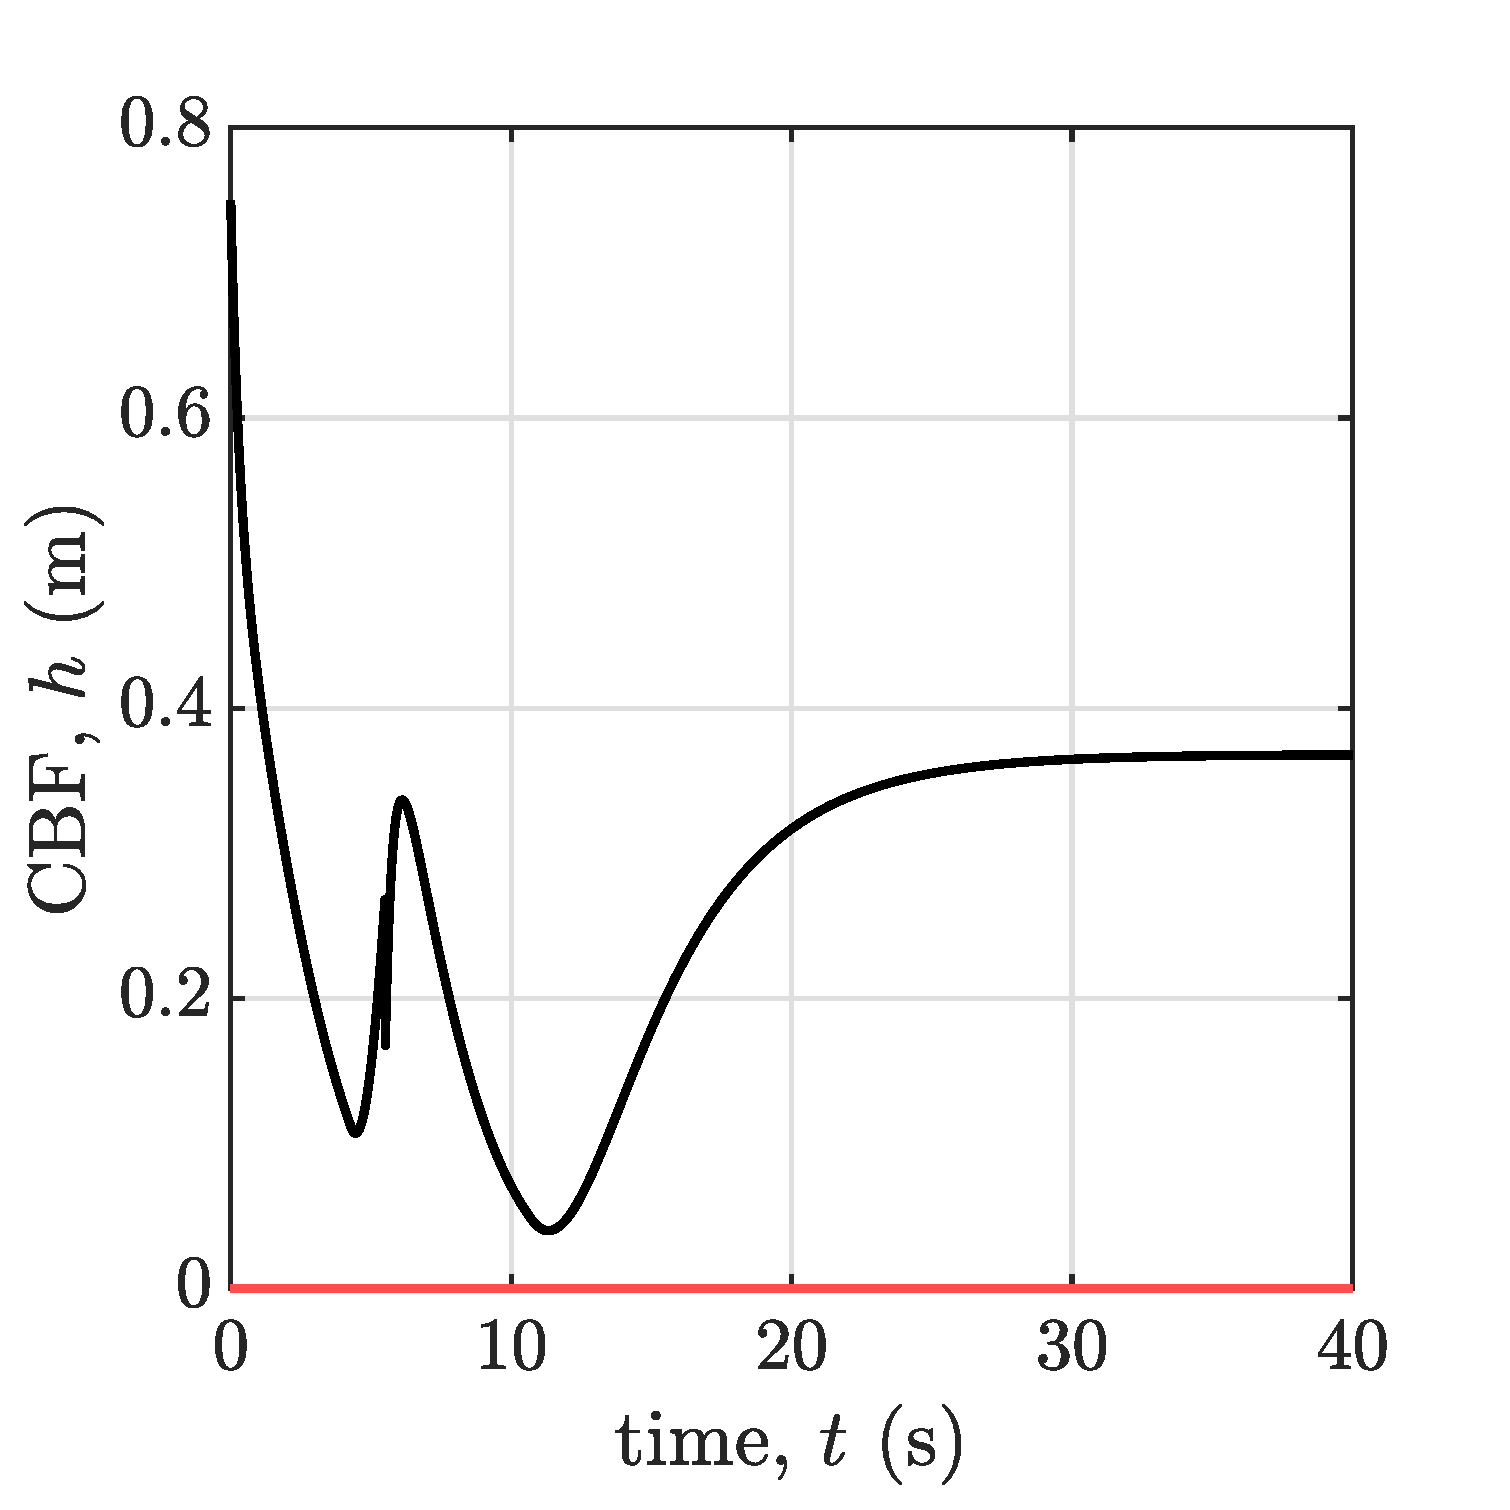
\includegraphics[width=\textwidth]{figures/sim3h.eps}
    \caption{\label{fig:sim3h}Sim 3: evolution of $h$.\\~}
    \end{minipage}
    \begin{minipage}[t]{.45\textwidth}
        \centering
        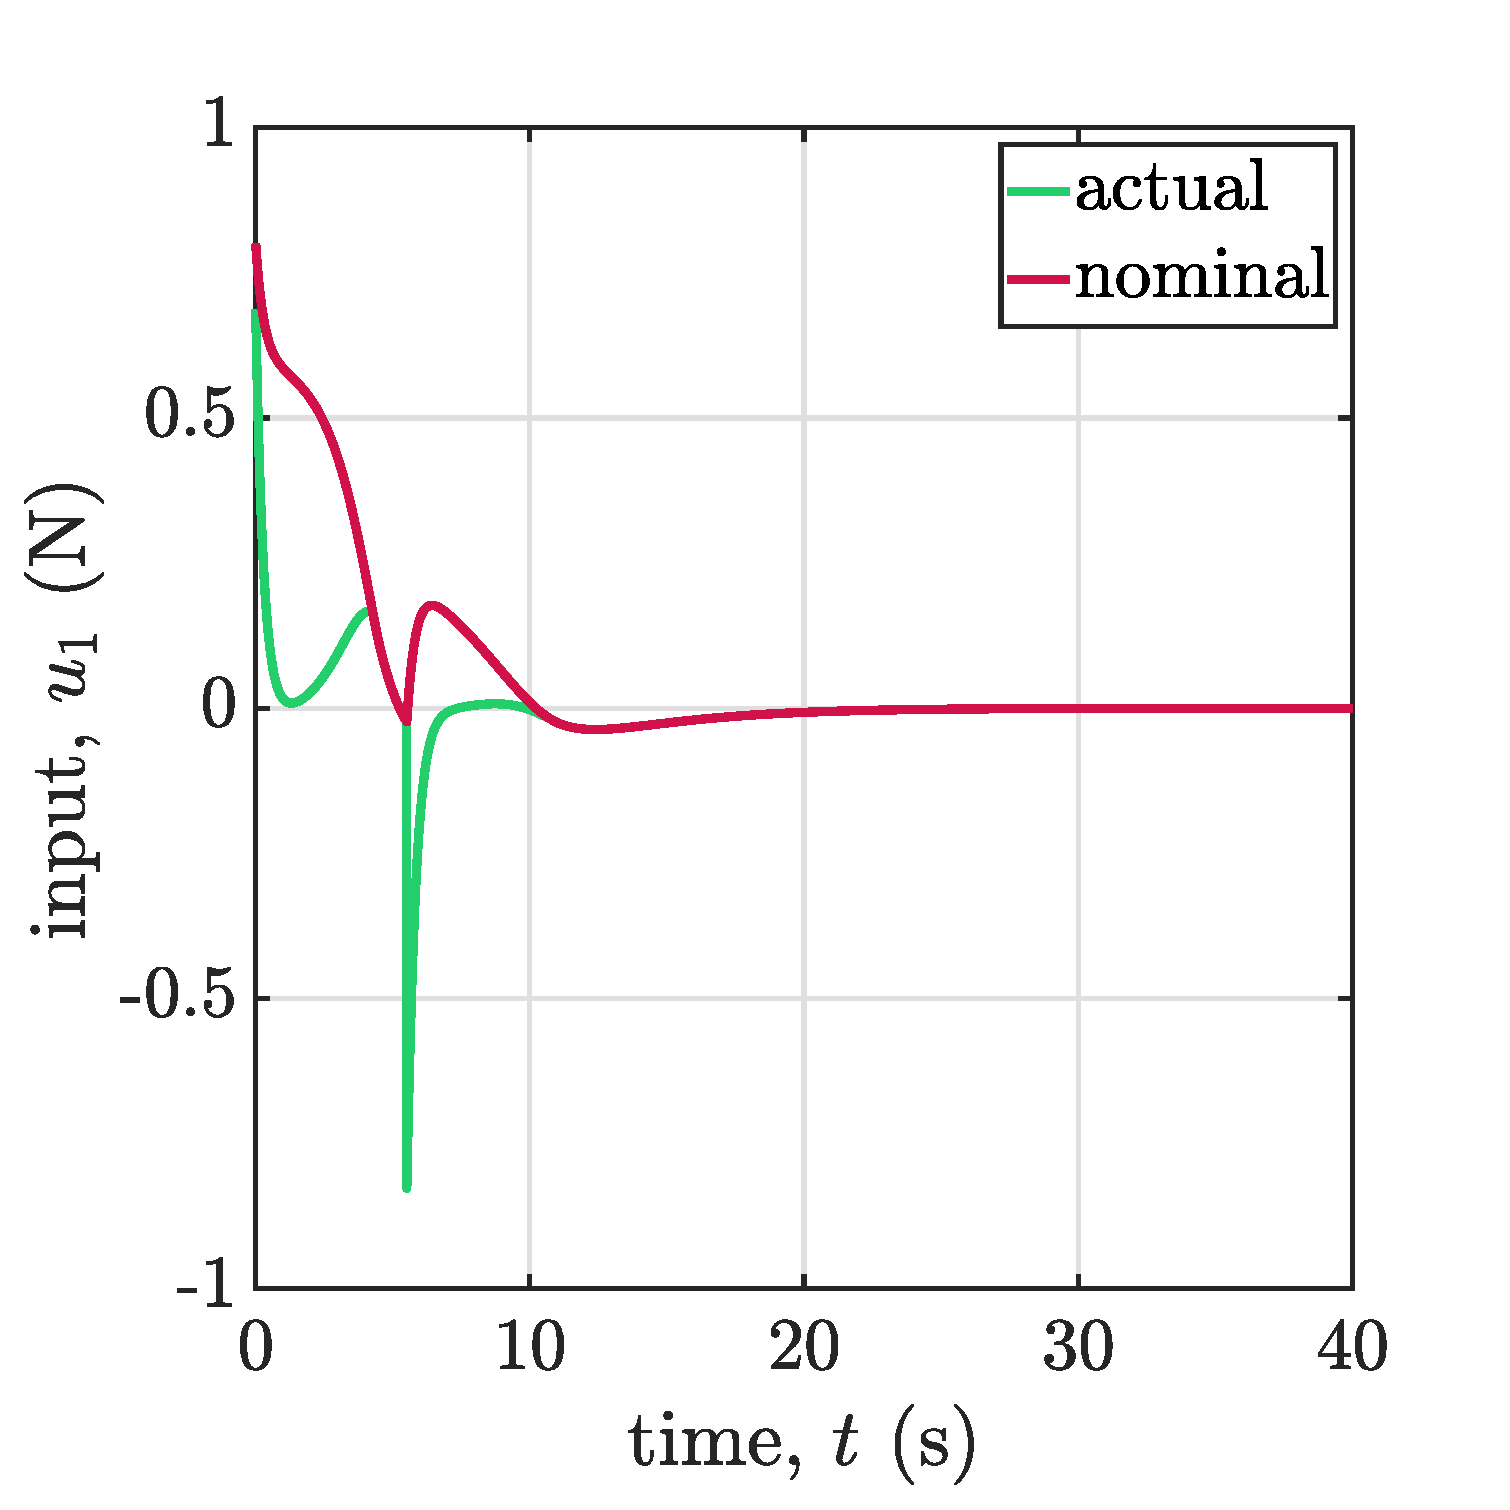
\includegraphics[width=\textwidth]{figures/sim3u1.eps}
    \end{minipage}
    \hfill
    \begin{minipage}[t]{.45\textwidth}
        \centering
        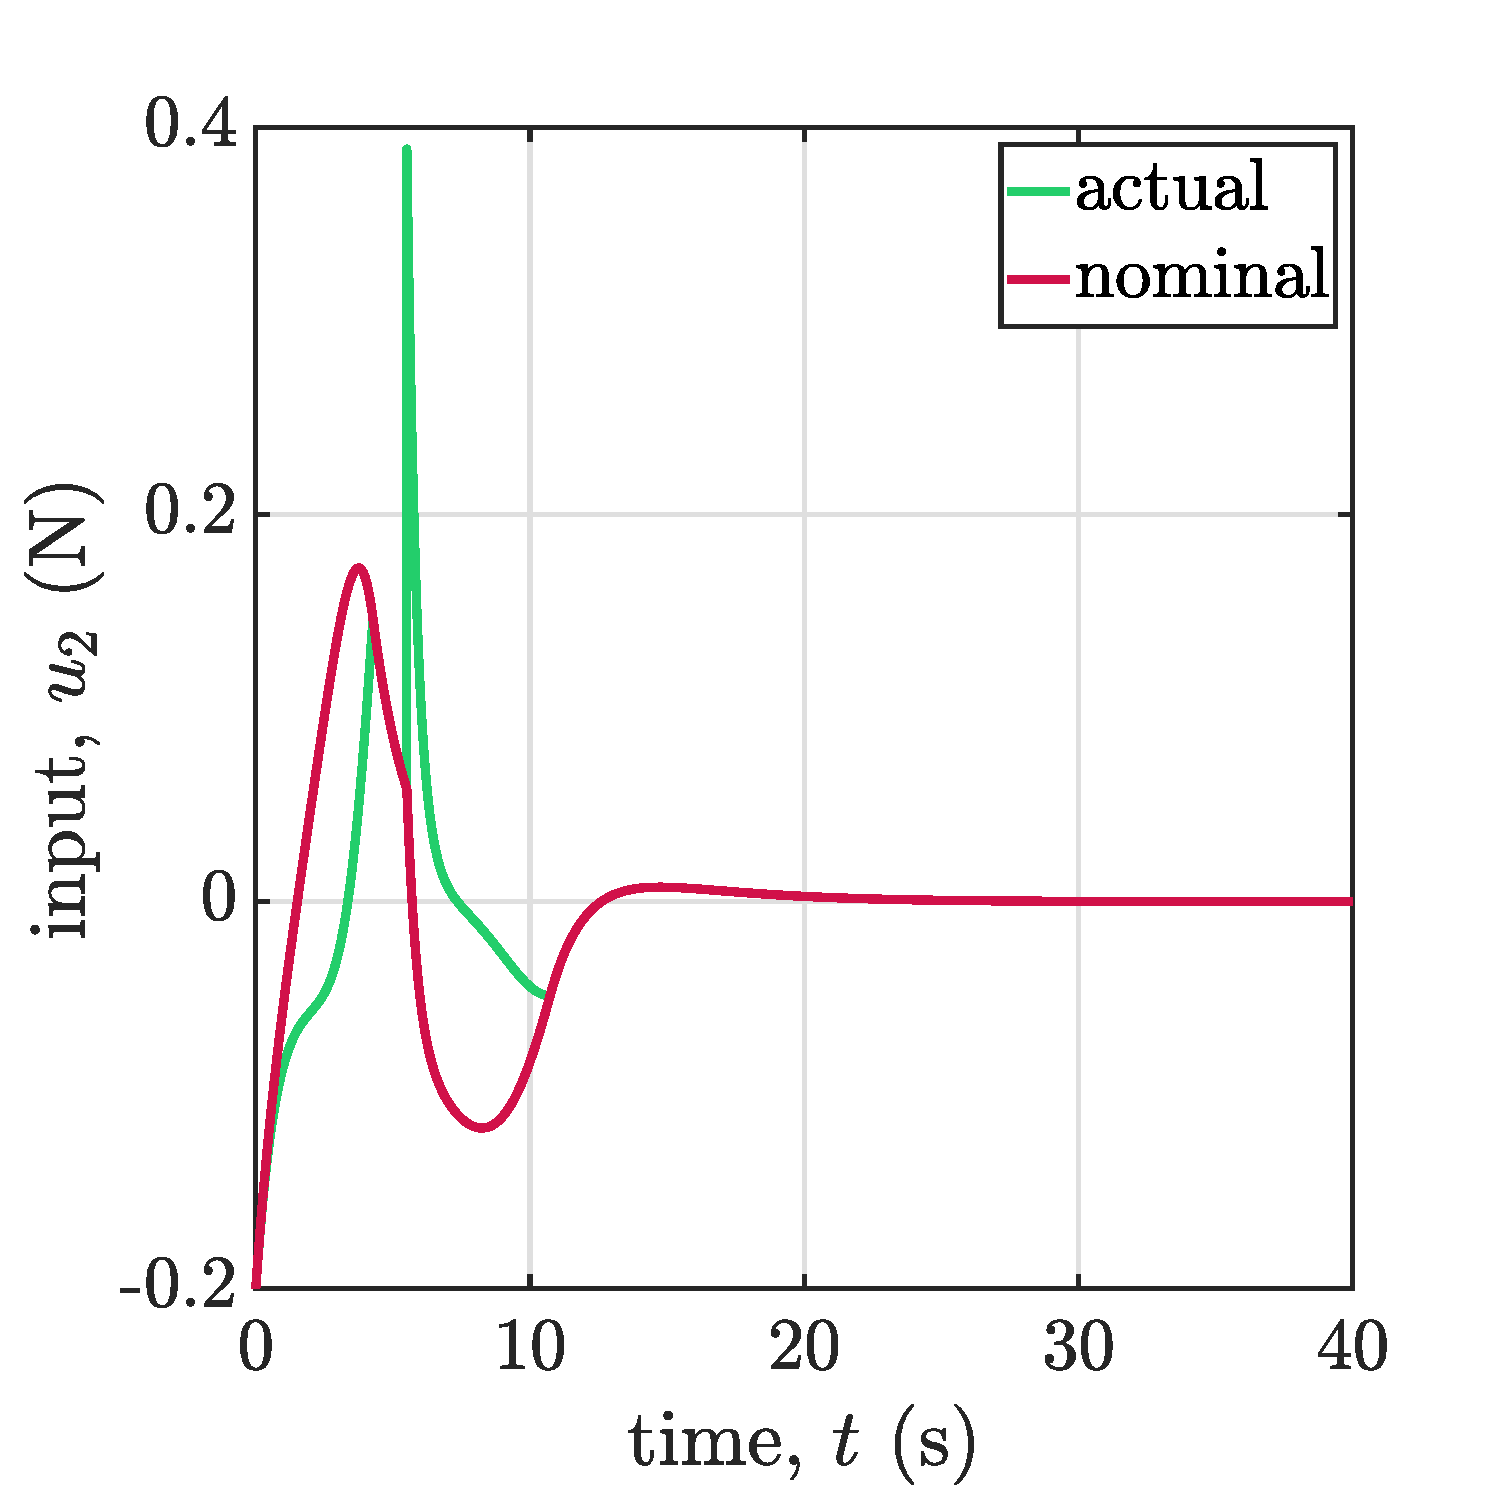
\includegraphics[width=\textwidth]{figures/sim3u2.eps}
    \end{minipage}
    \caption{\label{fig:sim3u} Sim 3: evolution of the input vector $\uv$ components}

\end{figure}
%add figure inputsim2 e input sim3
% Side by side figures 
%% unycycle !!
\subsection{Unicycle}
The other robotic system implemented is that of a circular body unicycle with $x$ and $y$ coordinates of a robot point along its sagittal axis at distance $|a|$ from the wheeel contact point. The dynamic model is given by
\begin{equation}
\left\{ \begin{aligned} \label{eq:dynUn}
    &\dot{x}      = v\cos\theta -\omega a\sin\theta \\
    &\dot{y}      =  v\sin\theta +\omega a\cos\theta \\
    &\dot{\theta} =  \omega \\
    &\dot{v}      =   1/m~u_1 \\
    &\dot{\omega}   = 1/I_{cm}~u_2 
\end{aligned} \right.
\end{equation}
\noindent
The choice of controlling point $a$ instead of the position of the wheel is made to ensure a fair comparison between the two approaches, in fact even though \eqref{eq:dynUn} can be feedback linearized when $a=0$, the kinematic model cannot without a change of coordinates or other strategies. This difference would result in an unequal comparison between the two approaches for the Cartesian regulation task being analyzed.
Regarding the CBF, for these simulations we aim to adopt a more sophisticated approach that can handle multiple obstacles more effectively. The current method of dealing with one obstacle at a time, during the CBF constraint evaluation may lead to discontinuities in $h$, as shown in Figure~\ref{fig:sim3h}. Additionally, the unicycle may not be able to avoid an obstacle if it is considered too late due to the kinematic constraint. One thing to notice is that in the following plots we represent the unicycle as a point while the radius of each obstacle is augmented with the radius of the robot $r$ plus the displacement $|a|$, so that if the trajectory of the point does not intersect any obstacle we can ensure no collisions. The unicycle parameters are $m=5.3$ [kg], $r=0.3$ [m], $I_{cm}=0.24$ [kg $\text{m}^2$], $a=0.1$ [m]. The unicycle starts at rest with pose $(\pv_{start}^T,\theta_{start})^T=(x_{start},y_{start},\theta_{start})^T = (0,0,\pi/2)^T$ and we want to reach $\pv_{goal}=(8,-3)^T$. In this case, the considered obstacles are $\pv_{\mathcal{O}_1}=(3.5,0.5)^T$, $\pv_{\mathcal{O}_2}=(3,-1.5)^T$, $\pv_{\mathcal{O}_3}=(6,-1)^T$ with radius $R_{\mathcal{O}_1}=0.45$, $R_{\mathcal{O}_2}=0.45$, $R_{\mathcal{O}_3}=0.75$ [m].

\subsubsection{Model-free CBF}
Let us consider  the first three components $\dqv$ of \eqref{eq:dynUn} i.e. its kinematic model. The velocity to reach the goal without taking into account any obstacles is
\begin{equation}\label{eq:qnominalu}
    \vv_{nom}= \begin{pmatrix}v_{nom} \\ \omega_{nom} \end{pmatrix} = -\begin{bmatrix}\cos\theta & \sin \theta\\ -\sin \theta /a & \cos \theta/a \end{bmatrix} K_P\cdot\boldsymbol{I}_{2} (\pv-\pv_{goal}), K_P \in \mathbb{R}_{>0},
\end{equation}
where $\pv$ and $\pv_{goal}$ are the cartesian coordinates of the robot and the goal respectively.
The CBF used to avoid obstacles is similar to \eqref{eq:cbfsim1} but with the inclusion of a term that considers if the system is moving towards the obstacle $\mathcal{O}_i$
\begin{equation}\label{eq:mfcbf2}
    h_i(\qv) = d_i-R_{\mathcal{O}_i}-\delta \cos(\theta - \psi_i),
\end{equation}
where $\psi_i= \arctan((y_{\mathcal{O}_i}-y)/(x_{\mathcal{O}_i}-x))$ is the robot-$\mathcal{O}_i$ angle and $\delta \in \mathbb{R}_{>0}$ is a tunable parameter. This CBF is highly effective for the unicycle as it encourages the robot to steer away from obstacles. In Simulation 4, we used multiple CBF constraints such that each component $i$ of $h(\qv) = (h_1(\qv),~...,~h_{l}(\qv))^T$ is defined as \eqref{eq:mfcbf2} and $l=3$ is the number of obstacles. 
Here, controller \eqref{eq:mf controller} tracks the safe velocity $\vv_{safe}$ from \eqref{eq:optprob} with $\Km_D=2.7\cdot\boldsymbol{I}_{2}$, then we set $K_P=0.1$, $\alpha = 0.50<\lambda=0.51,~\delta=2$ and bound $\dvv_{safe} \leq 0.5$. As shown in Figure~\ref{fig:sim4map}--\ref{fig:sim4h} the unicycle is capable of reaching its destination, but it has to circumvent the obstacles as the clearance, in this case, is $\gamma=1.45$ [m]. In Figure~\ref{fig:sim4v} we can see how the nominal angular velocity generated tries to align the robot with the goal, but due to the safety mechanism that prevents pointing in the direction of the obstacle, a much lower command is produced making the robot take a longer route. Anyway, it is worth noticing how increasing $\Km_{\!D}$ eigenvalues to reduce the clearance almost gives perfect tracking.
%Having an higher $K_D$ to bound $\gamma$ we are able to track very well this velocity.
%parlare di come tracka bene w visto che è piccolo Icm ma contribisce ad aumentare gamma perché l'eigenvalue di (17) è piccolo + gain aumentati per diminuire clearance
\subsubsection{Model-based CBF}
In the classic approach for Simulation 5, similar to the point robot, we cannot use directly \eqref{eq:ffcbf2} for each obstacle $\mathcal{O}_i$, but we need to add a term to have the relative degree equal to one. Using the same term added in \eqref{eq:difmcbf} the new CBF is:
\begin{equation}
   h_i(\qv,\dqv) = d_i-R_{\mathcal{O}_i}-\delta \cos(\theta - \psi_i)+\mu(\pv-\pv_\mathcal{O})^T\dpv
   \label{eq:ffcbf2}
\end{equation}
with $\pv$ the cartesian position vector. In Simulation 5, we have generated $\uv_{nom}$ analogously to \eqref{eq:qnominalu} so that the system is linearized and a simple PD controller can be employed
    \begin{equation}
          \uv_{nom}= \begin{pmatrix}
      \cos\theta/m & -a\sin\theta/I_{cm} \\
       \sin\theta/m & a\cos\theta/I_{cm}
    \end{pmatrix}^{-1} 
     \begin{bmatrix}
     - \begin{pmatrix}
     -v\omega\sin\theta-\omega^2a\cos\theta \\
        v\omega\cos\theta-\omega^2a\sin\theta
         \end{pmatrix}
           + \ddpv_{nom}
         \end{bmatrix},
    \end{equation}
with  $\ddpv_{nom} = -\Km_P(\pv-\pv_{goal})-\Km_D~\dpv$. By solving the multi-CBF optimization problem for the same obstacles in Simulation 4 we produce the $\uv_{safe}$, which is given directly in input to the model. Setting $\Km_P = 0.2\cdot\boldsymbol{I}_2,$ $\Km_D = \boldsymbol{I}_2,$ $\delta = 0.2$, $\alpha = 0.8$, $\mu = 0.3$, the robot is now able to pass in between the obstacles Figure~\ref{fig:sim5map} to reach the goal since it does not need additional clearances to ensure safety.
 % Simulation 4 
\begin{figure}[!ht]
    \begin{minipage}[b]{0.46\linewidth}
    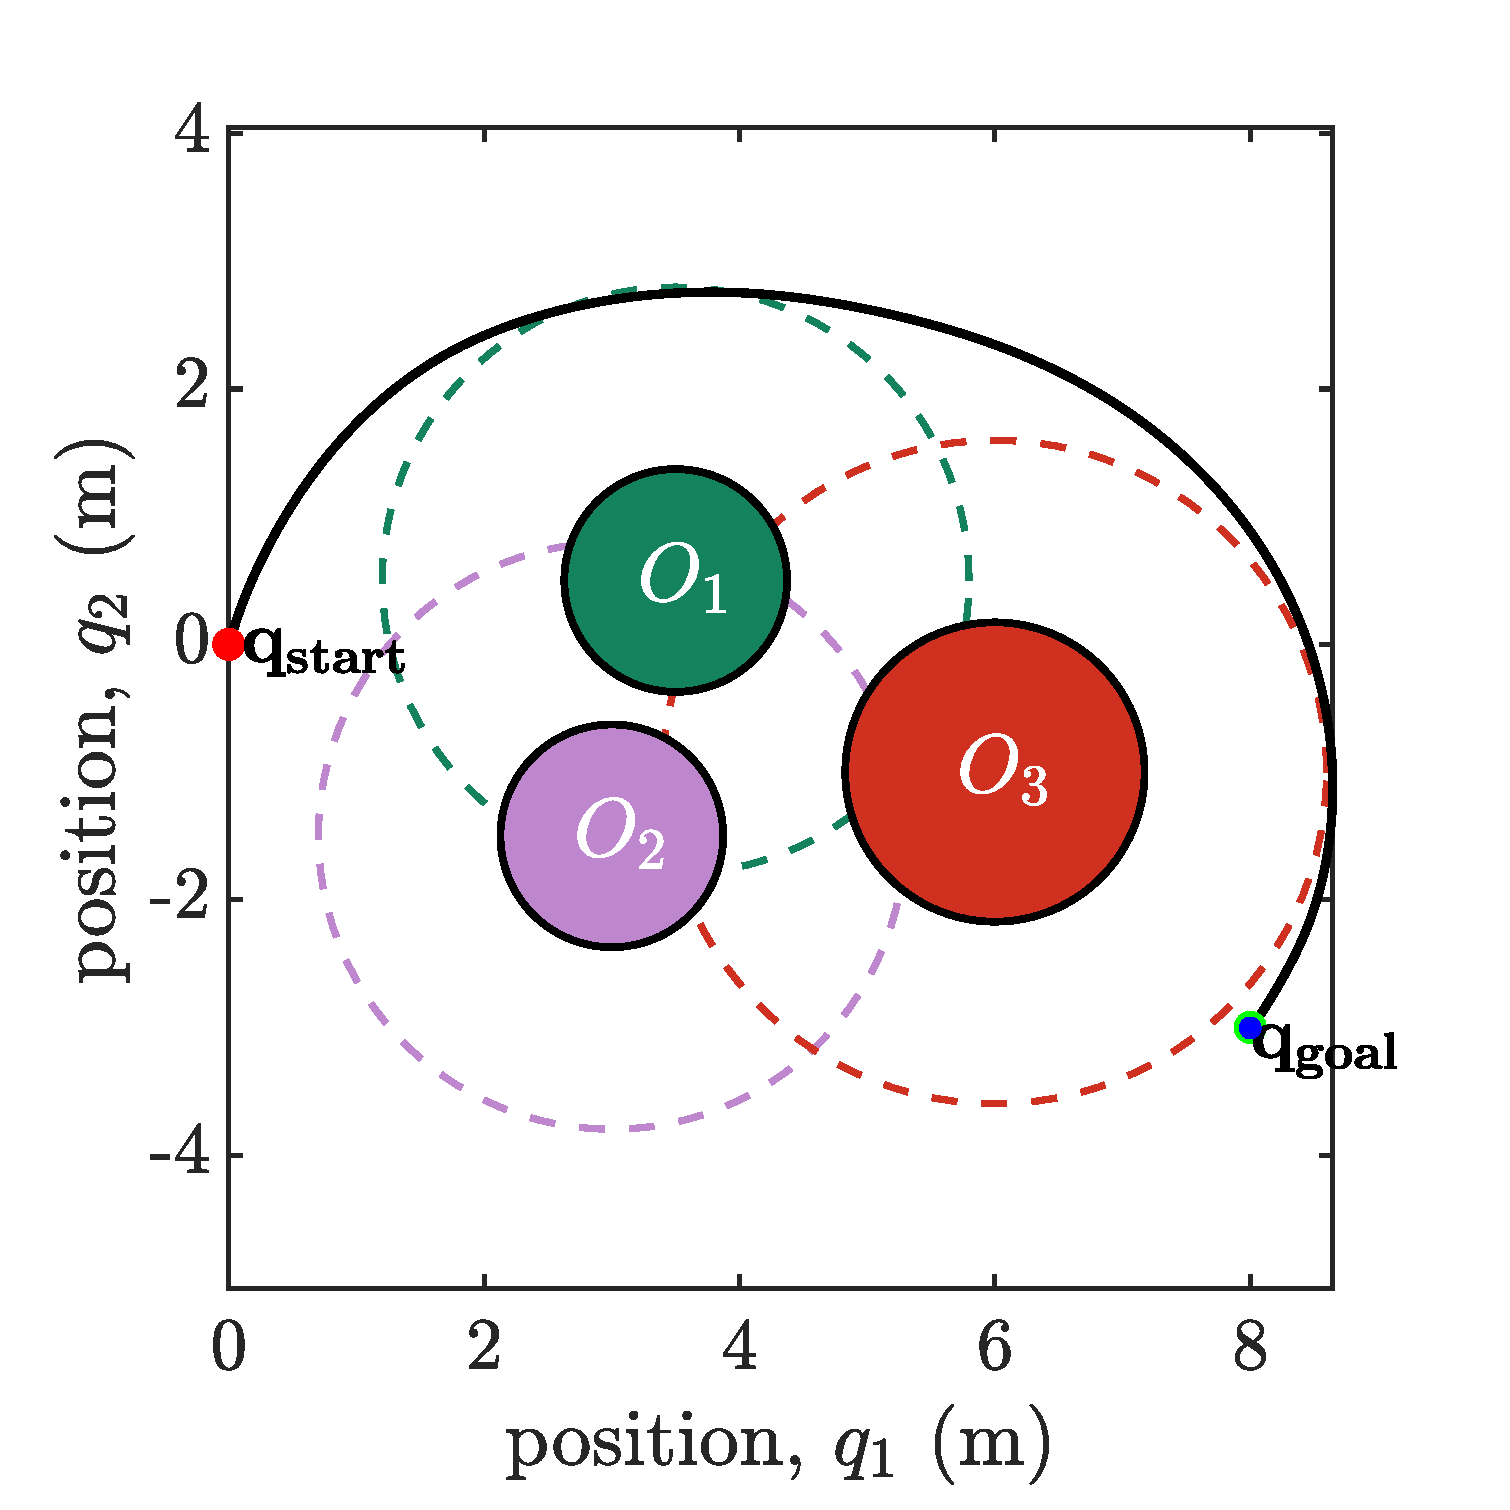
\includegraphics[width=\textwidth]{figures/sim4map.eps}
    \caption{\label{fig:sim4map}Sim. 4: evolution of the state $\qv$ over the environment.}
    \end{minipage}
    \hfill
    \begin{minipage}[b]{0.46\linewidth}
    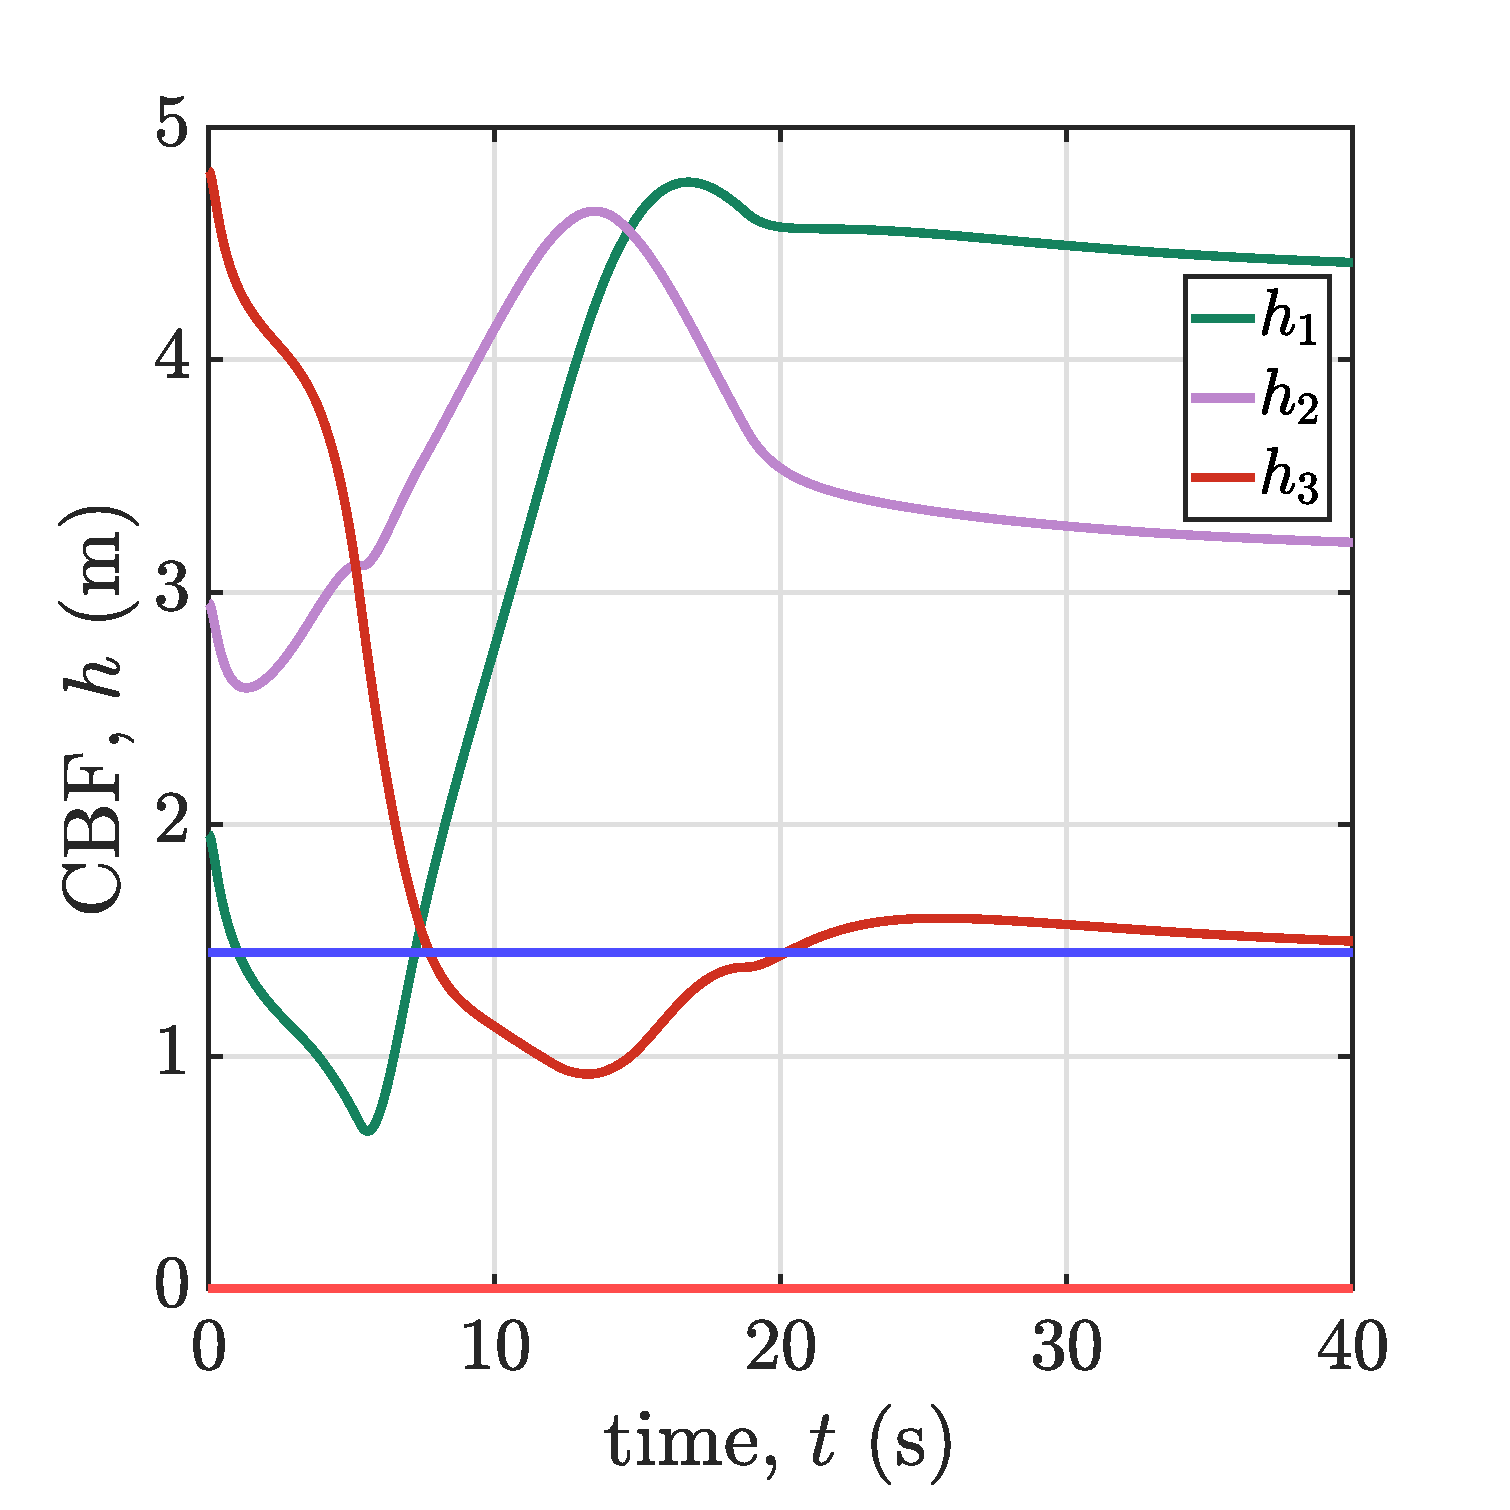
\includegraphics[width=\textwidth]{figures/sim4h.eps}
    \caption{\label{fig:sim4h}Sim 4: evolution of $h$ with $\gamma = 1.45\,[\mathrm{m}$] (blue line).}
    \end{minipage}
\end{figure}
\begin{figure}[!ht]
    \begin{minipage}[t]{.45\textwidth}
        \centering
        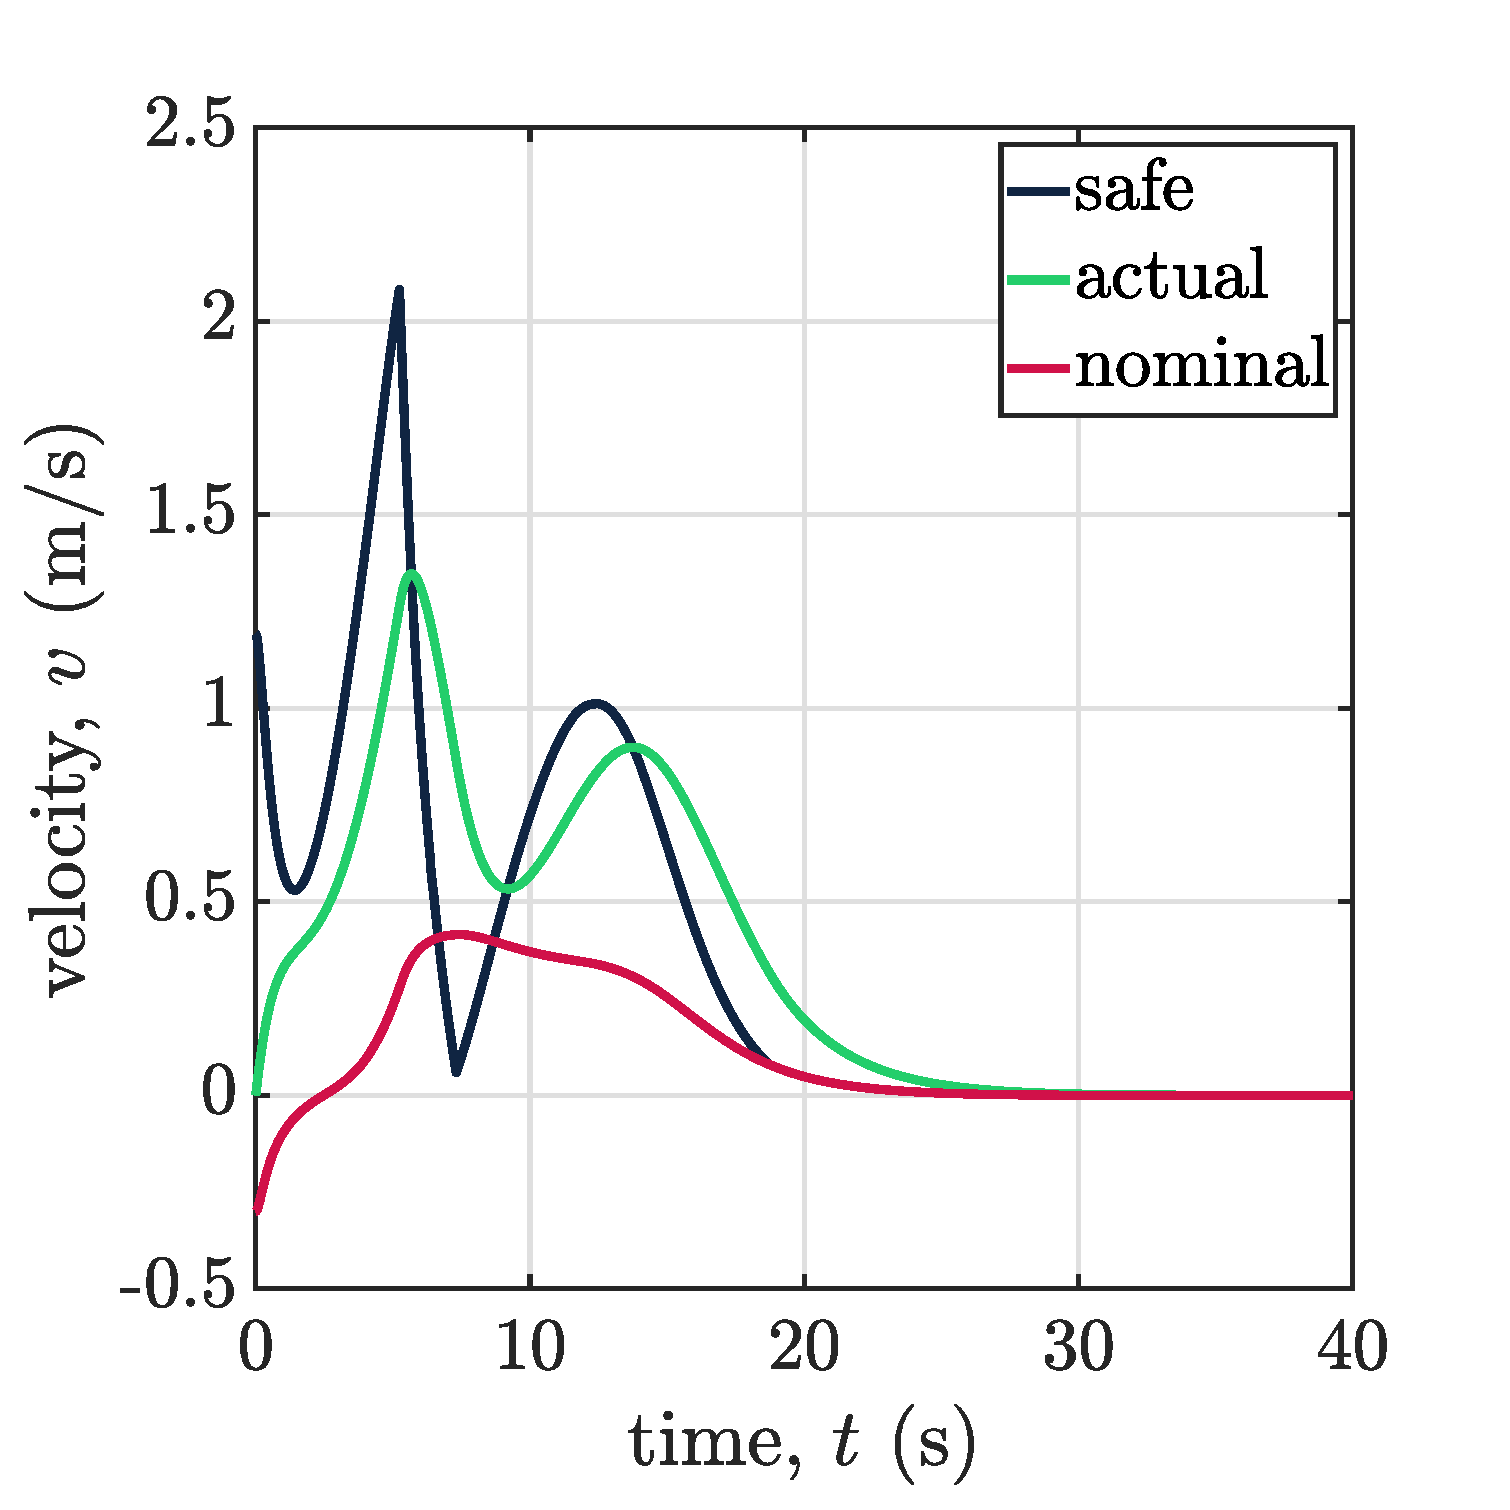
\includegraphics[width=\textwidth]{figures/sim4v1.eps}
    \end{minipage}
    \hfill
    \begin{minipage}[t]{.45\textwidth}
        \centering
        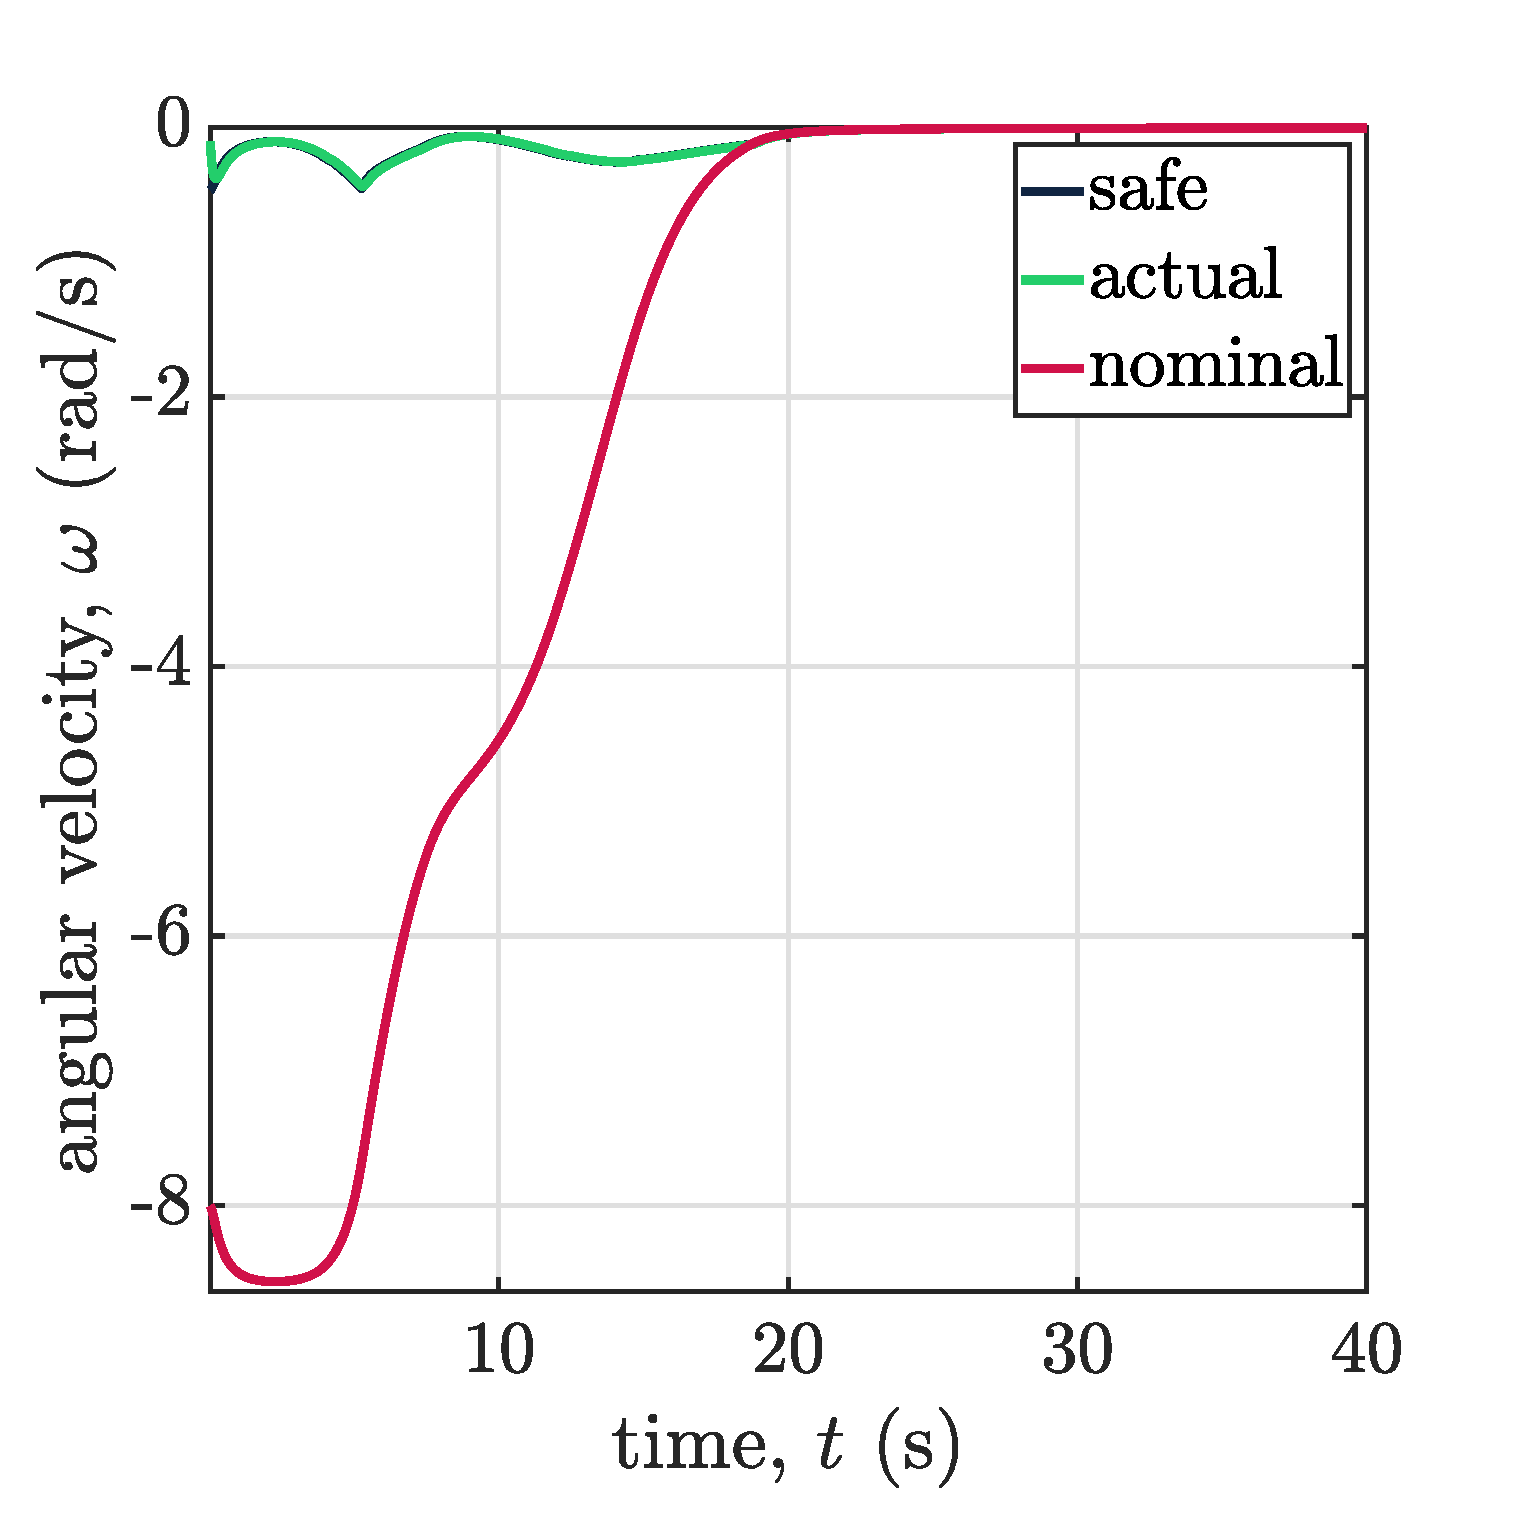
\includegraphics[width=\textwidth]{figures/sim4v2.eps}
    \end{minipage}  
    \caption{\label{fig:sim4v}Sim 4: Evolution of the velocity vector $\dqv$ components}
    
    \begin{minipage}[t]{.45\textwidth}
        \centering
        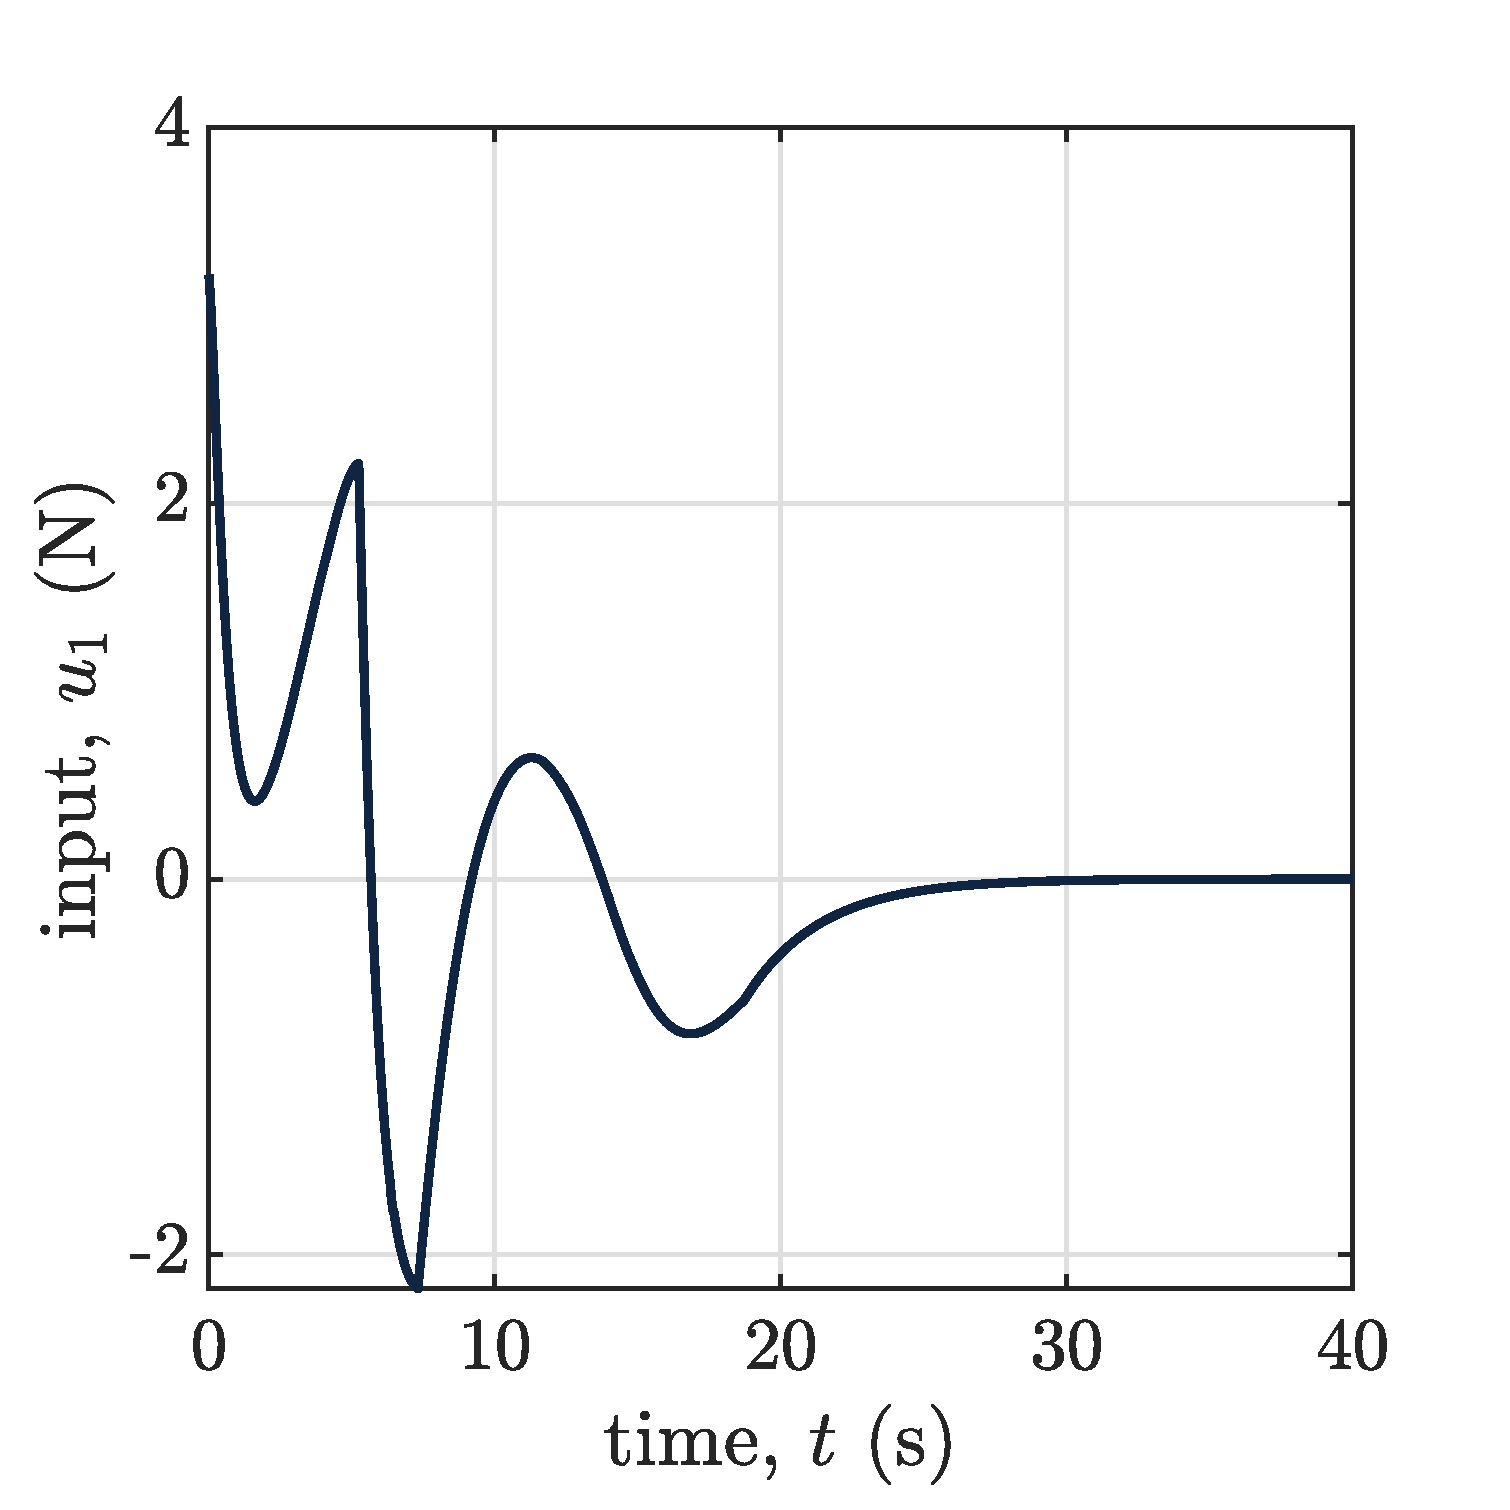
\includegraphics[width=\textwidth]{figures/sim4u1.eps}
    \end{minipage}
    \hfill
    \begin{minipage}[t]{.45\textwidth}
        \centering
        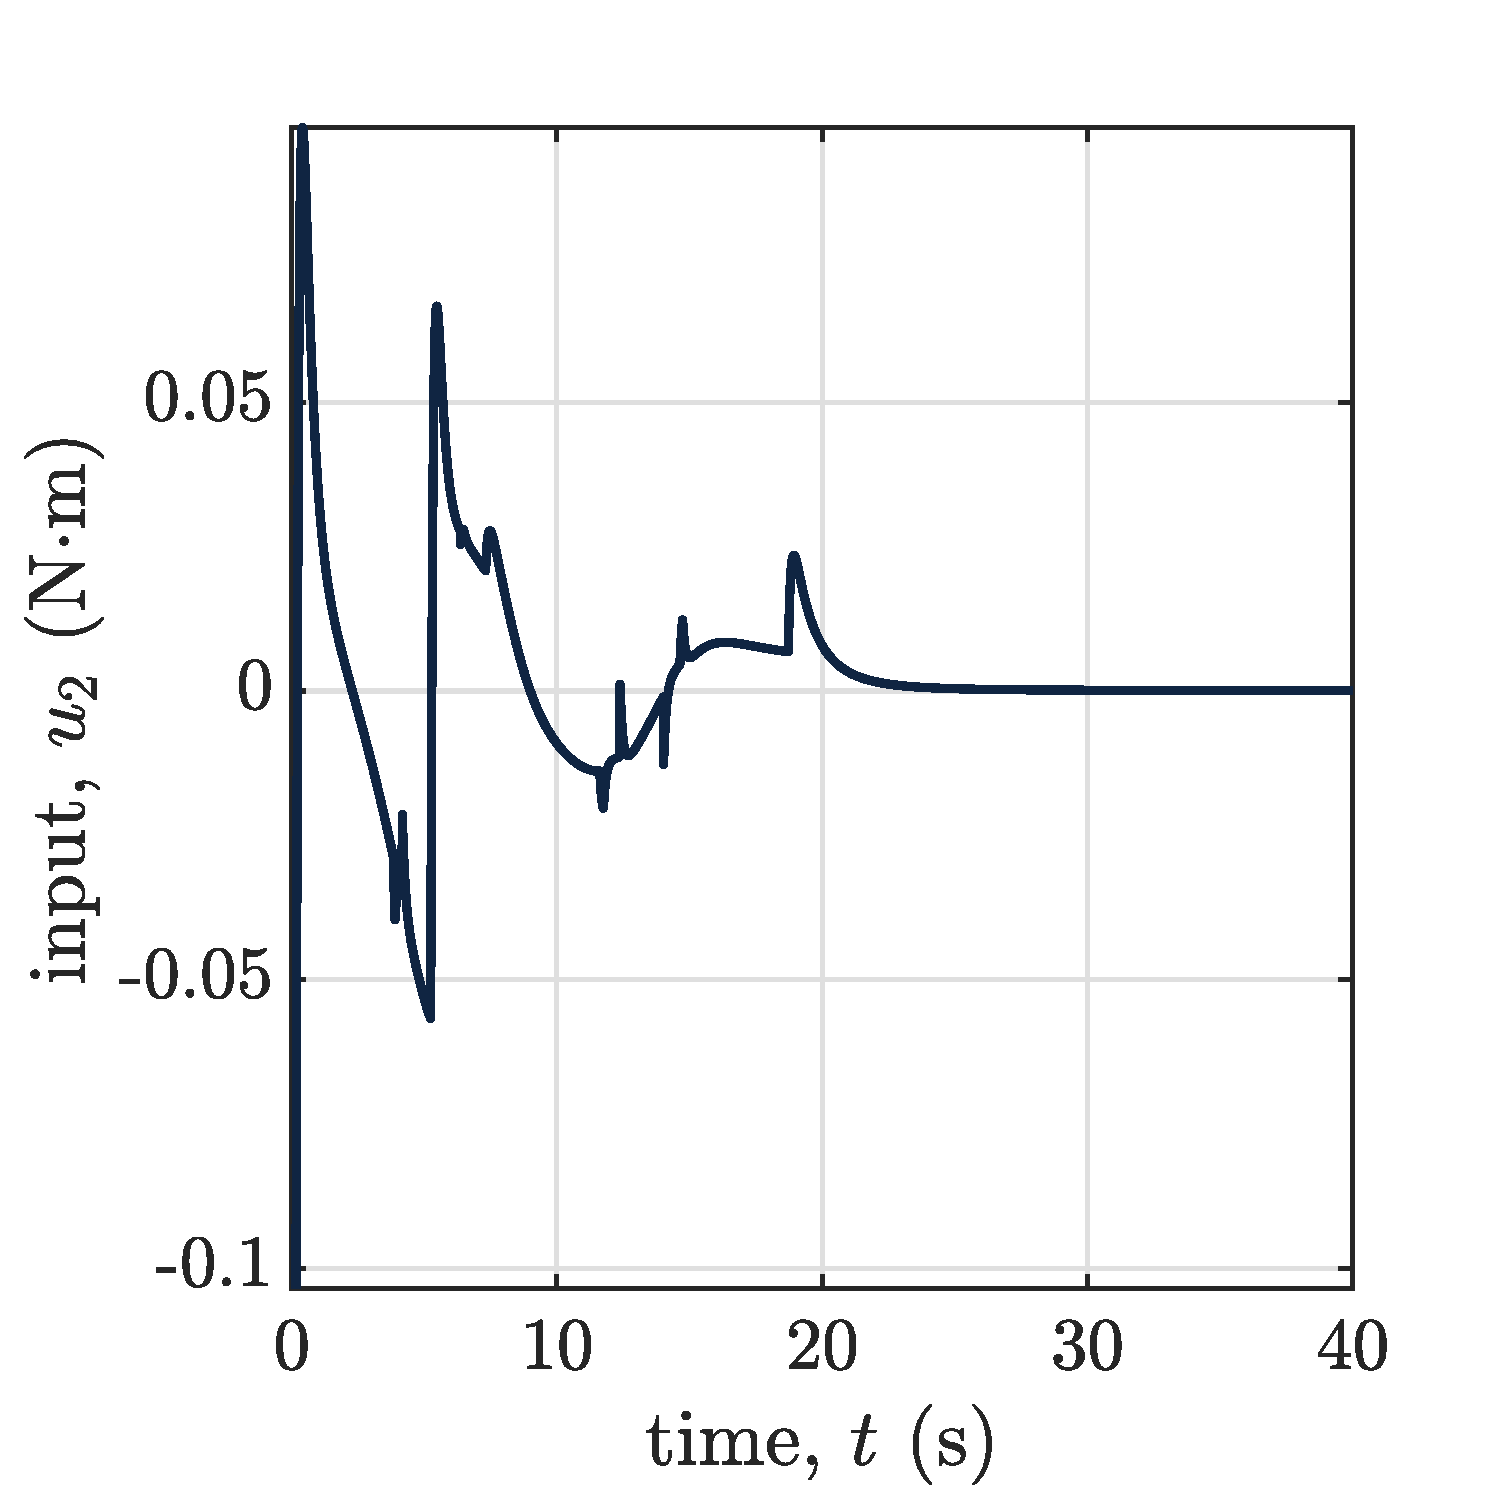
\includegraphics[width=\textwidth]{figures/sim4u2.eps}
    \end{minipage}  
    \caption{\label{fig:sim4u} Sim 4: Evolution of the input vector $\uv$ components}
    % Simulation 5
    \begin{minipage}[b]{0.46\linewidth}
    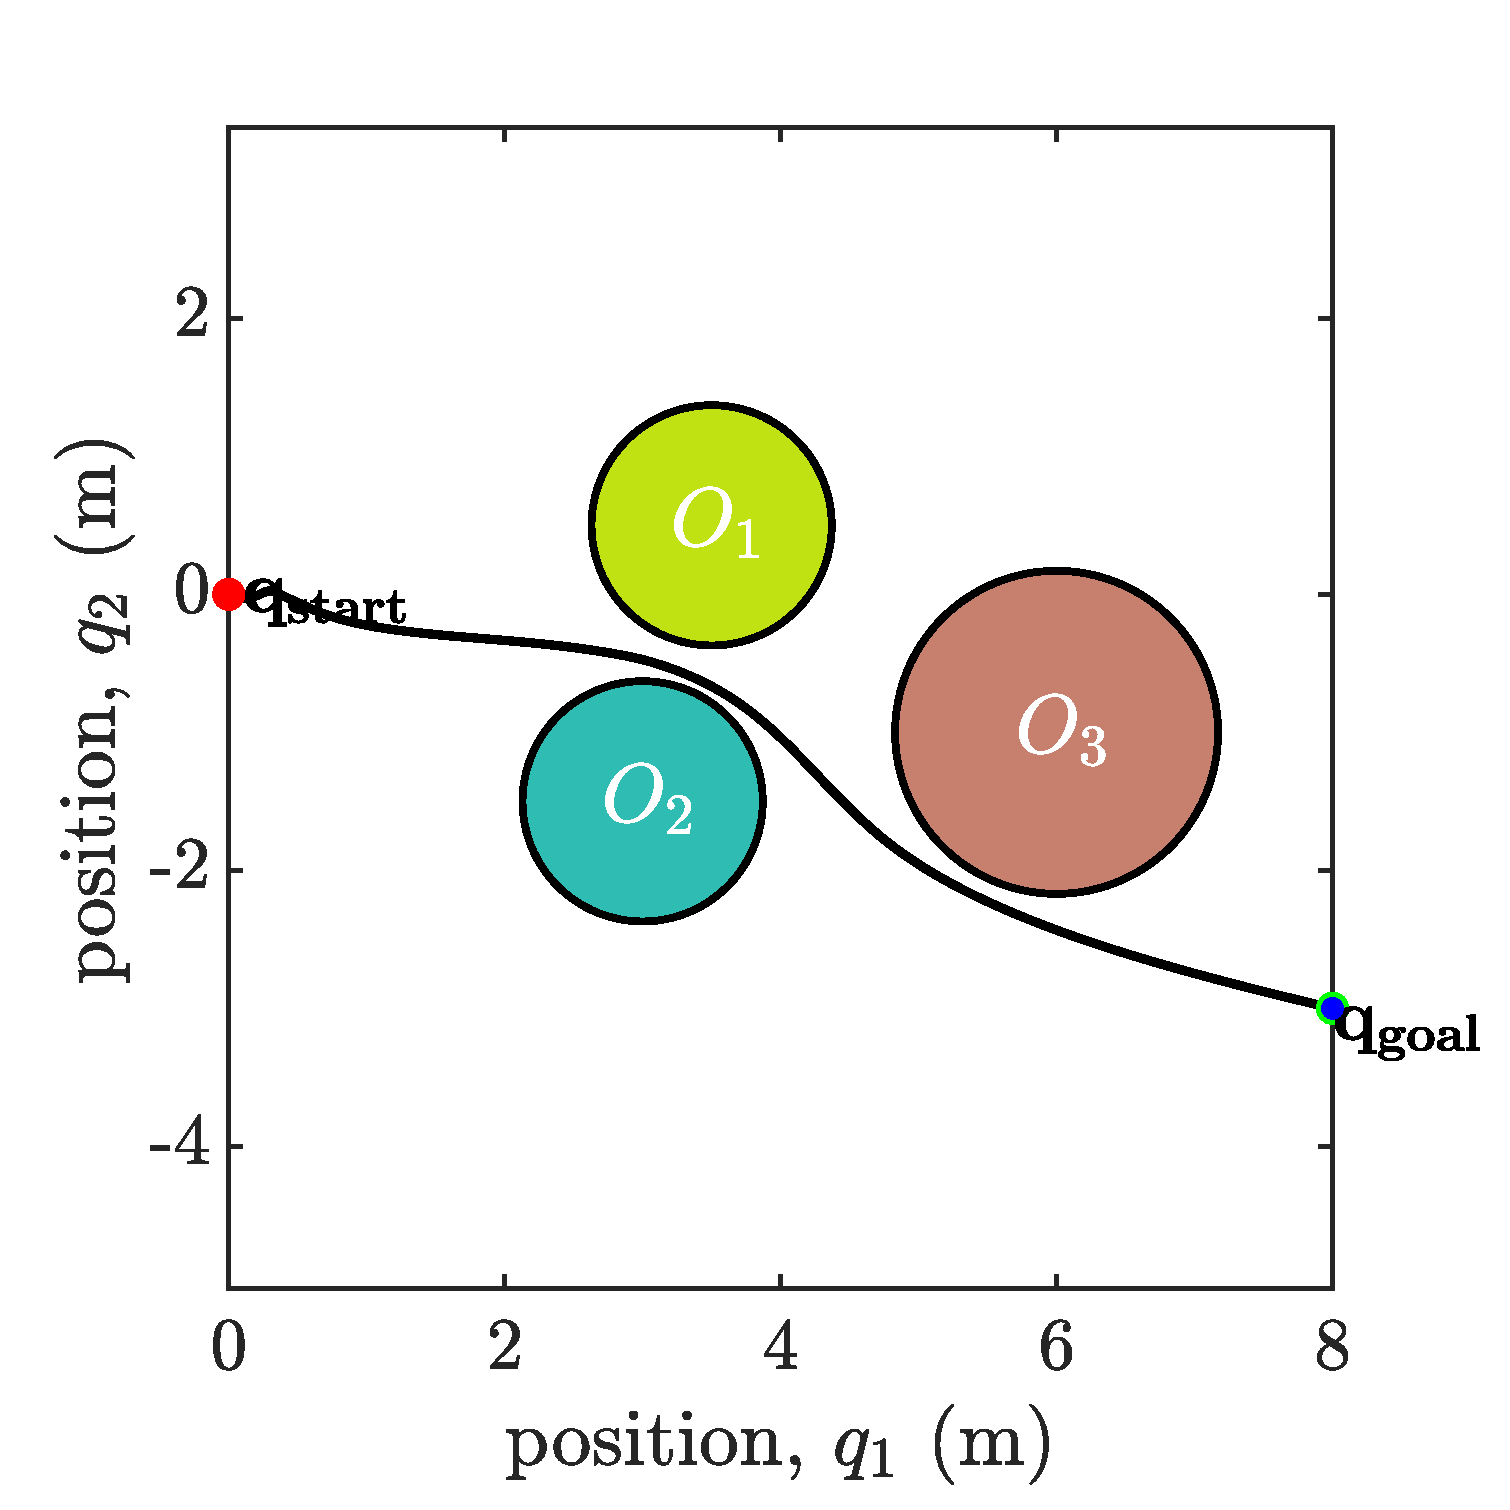
\includegraphics[width=\textwidth]{figures/sim5map.eps}
    \caption{\label{fig:sim5map}Sim. 5: evolution of the state $\qv$ over the environment.}
    \end{minipage}
    \hfill
    \begin{minipage}[b]{0.46\linewidth}
    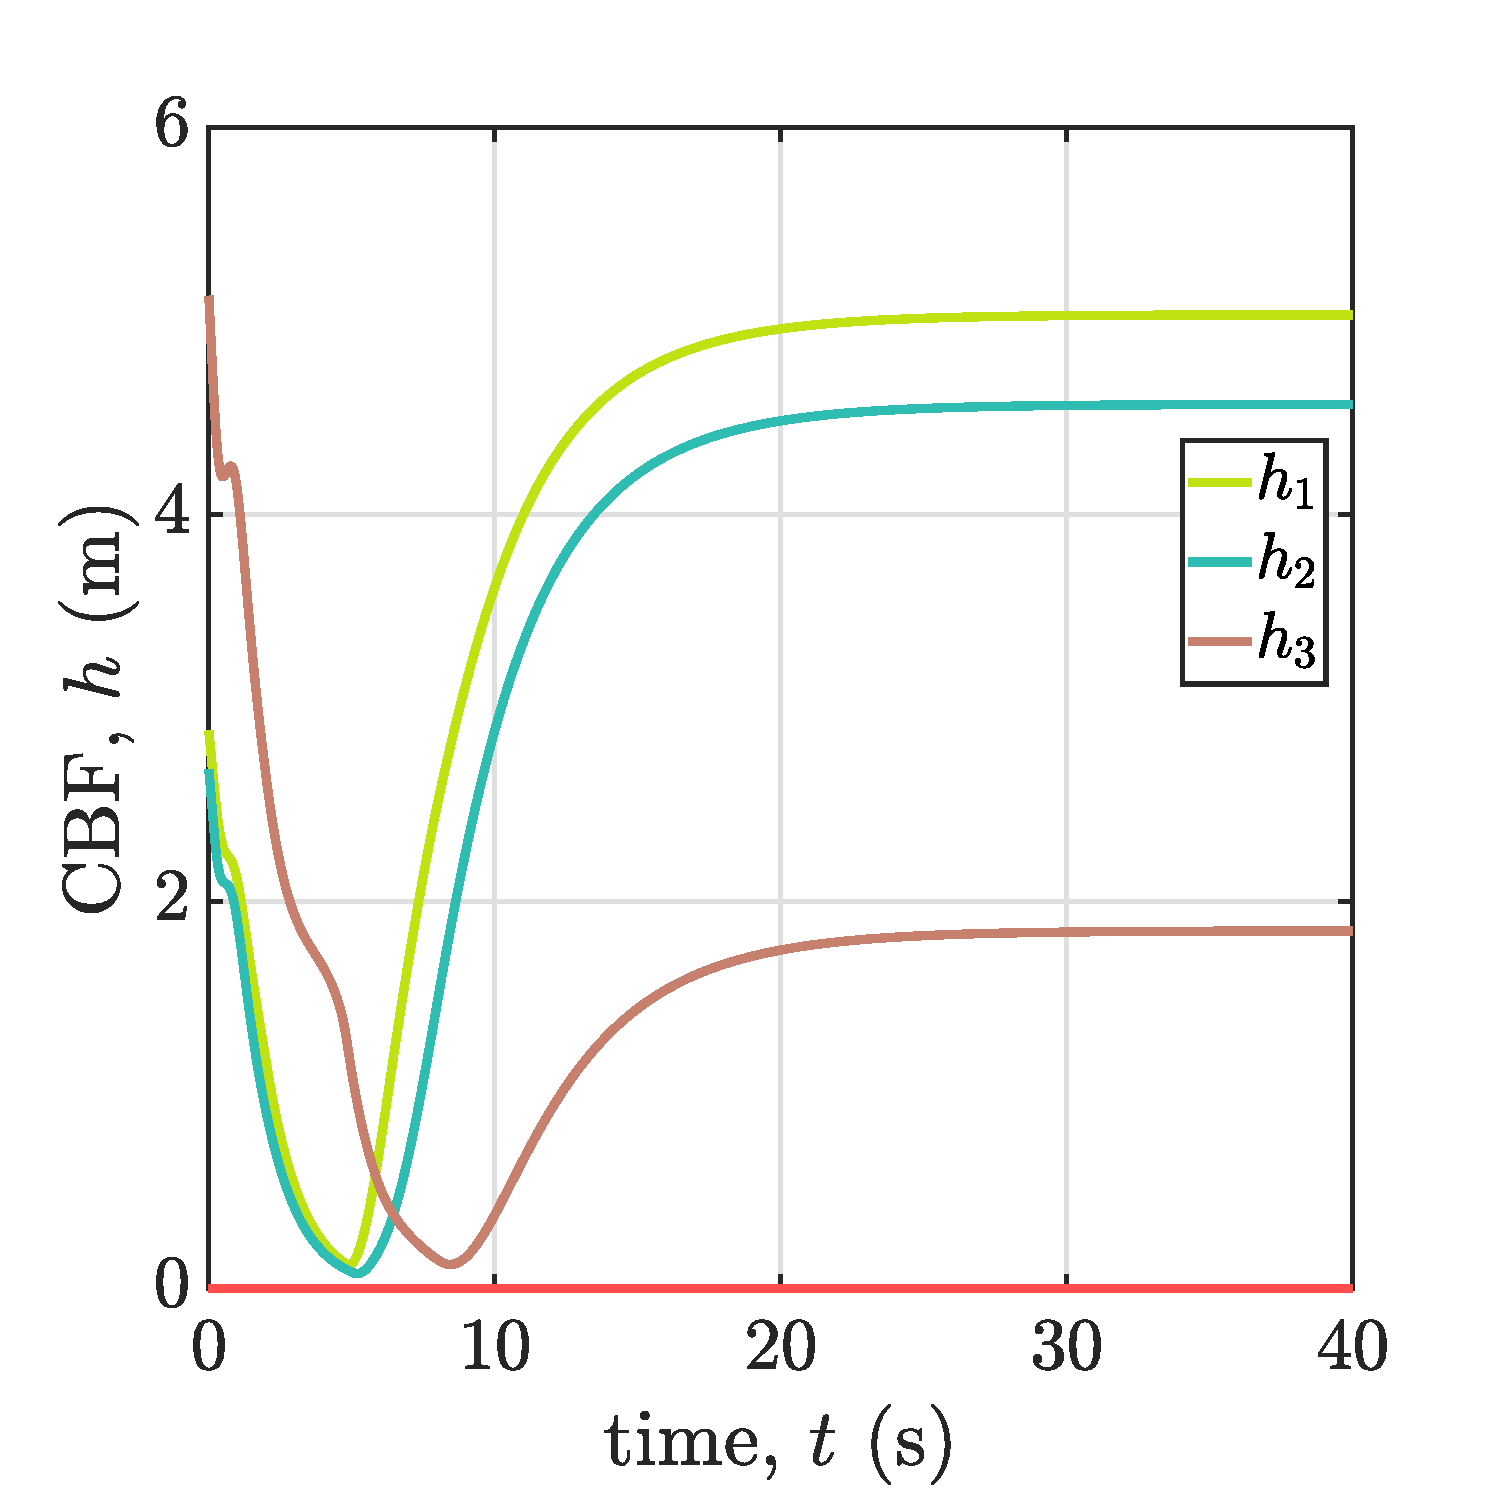
\includegraphics[width=\textwidth]{figures/sim5h.eps}
    \caption{\label{fig:sim5h}Sim 5: evolution of $h$.\\~}
    \end{minipage}
\end{figure}
\clearpage

\begin{figure}[!ht]
    \begin{minipage}[t]{.45\textwidth}
        \centering
        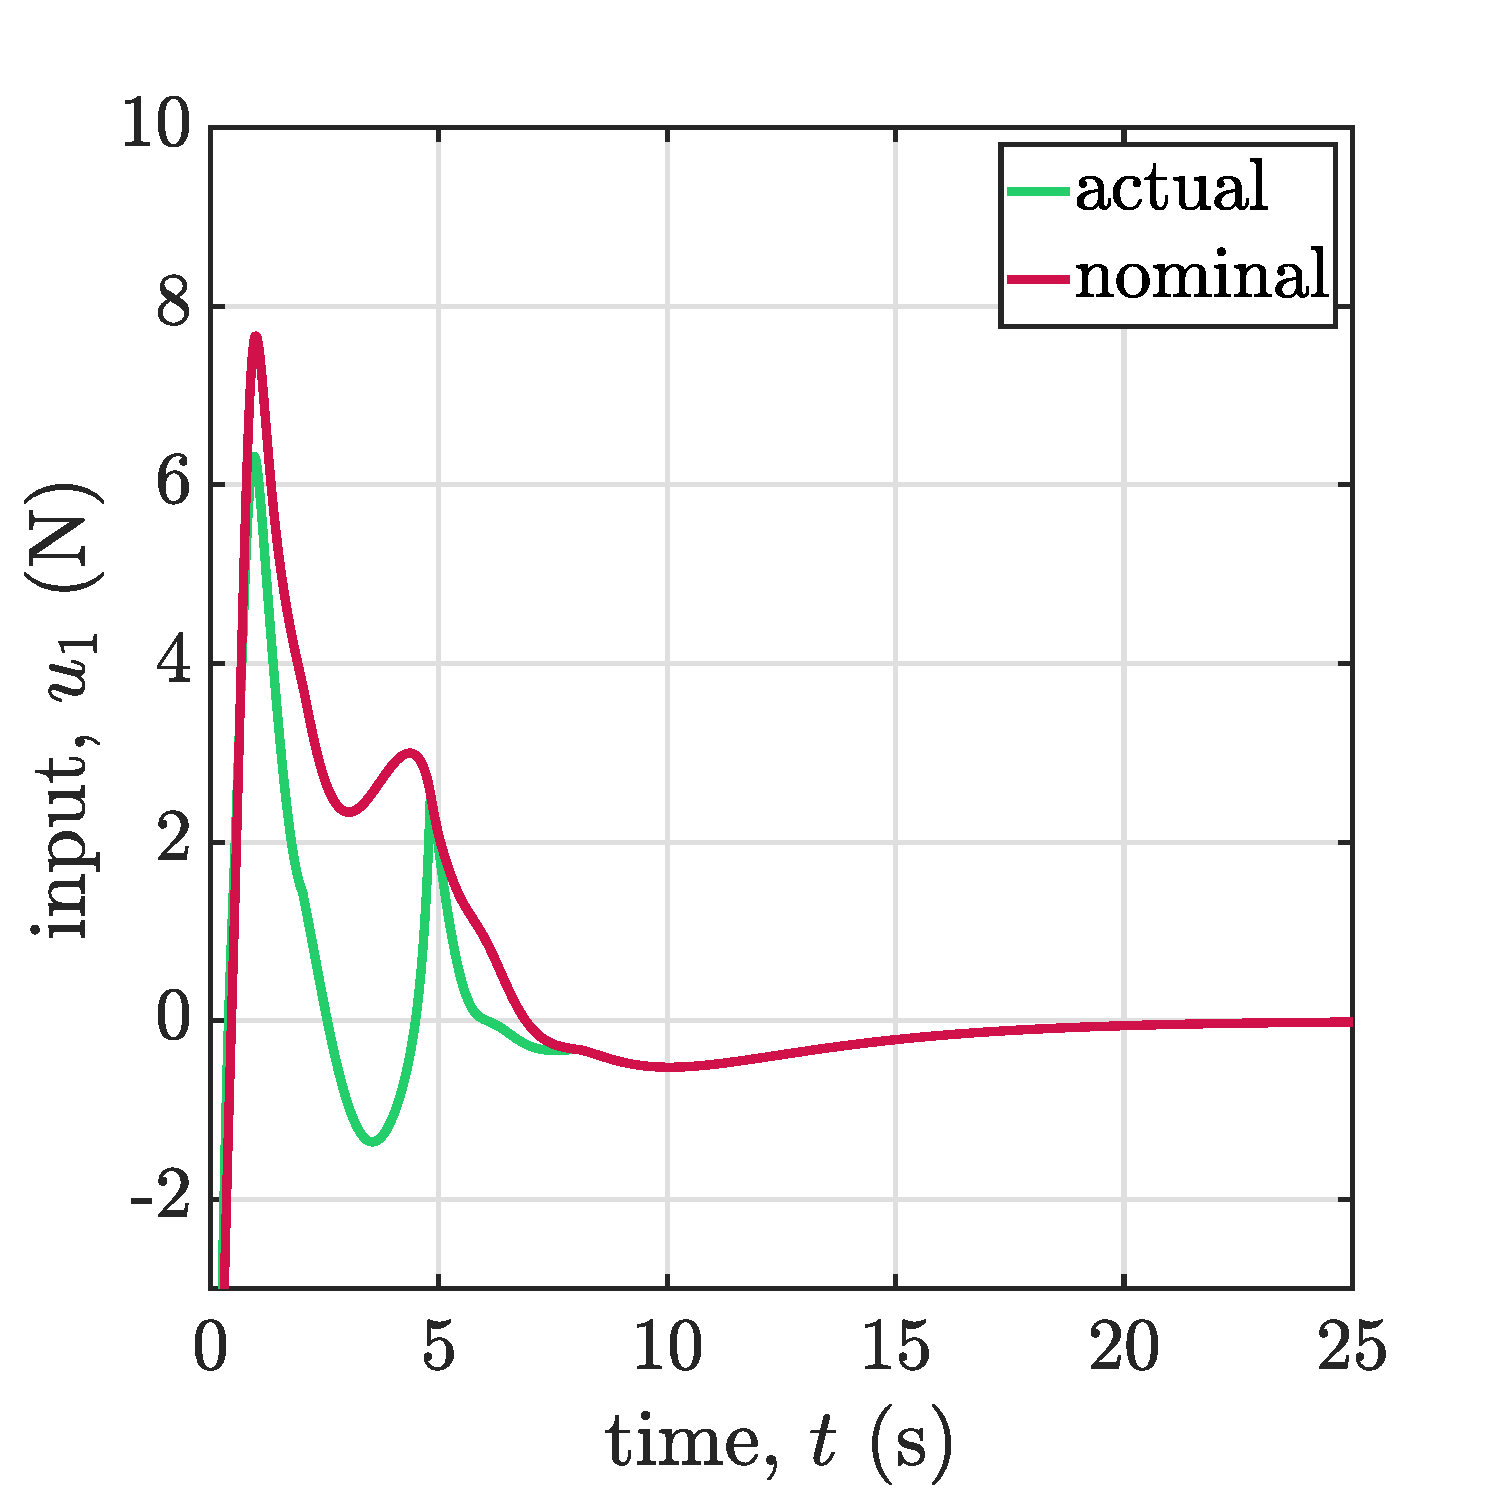
\includegraphics[width=\textwidth]{figures/sim5u1.eps}
    \end{minipage}
    \hfill
    \begin{minipage}[t]{.45\textwidth}
        \centering
        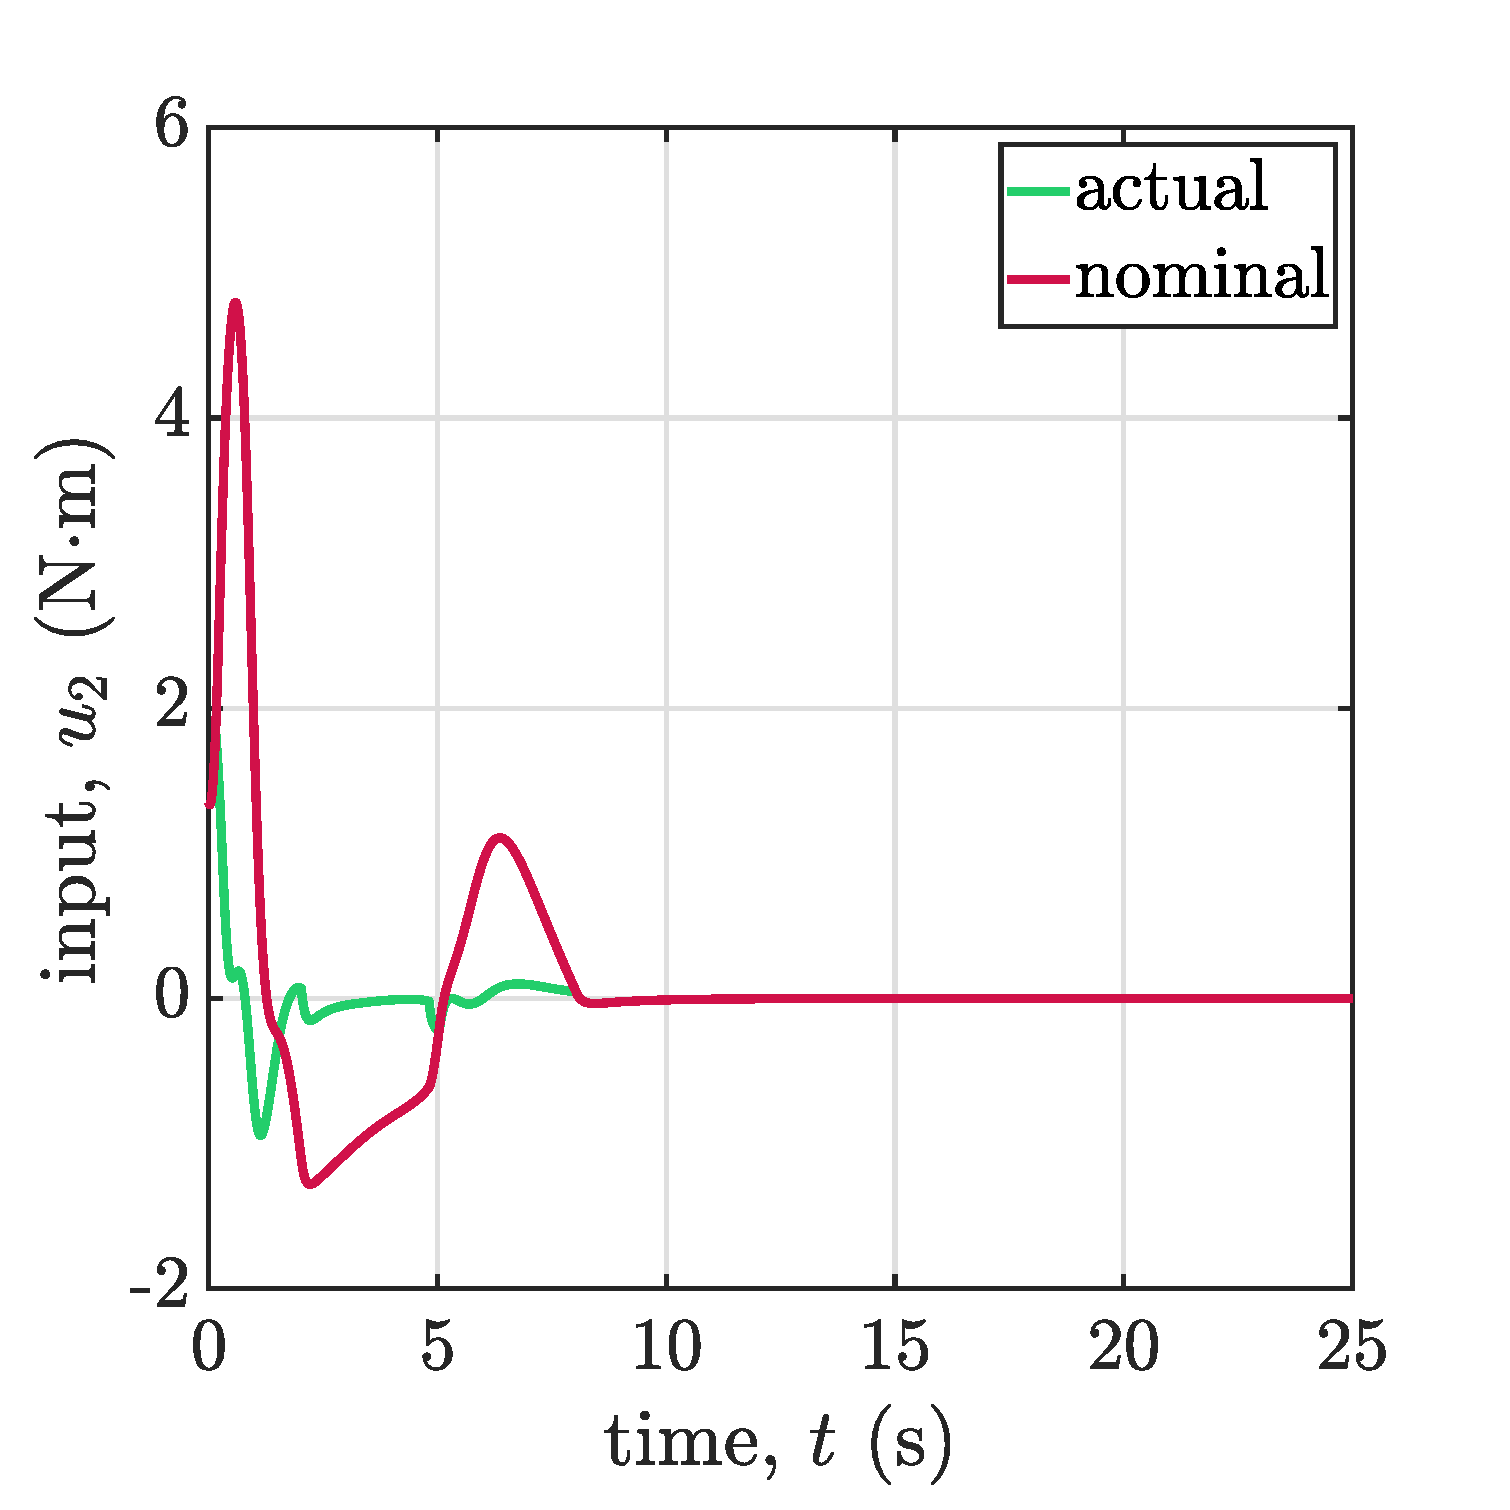
\includegraphics[width=\textwidth]{figures/sim5u2.eps}
    \end{minipage}
    \caption{\label{fig:sim5u2} Sim 5: evolution of the input vector $\uv$ components}
\end{figure}

% m=1 tutto come loro, m=15 sbanda senza "disturbo", m=15 con disturbo + 2 sim con cbf normale usando quella di venditelli
% \begin{align}
%     &\argmin_{\dot{\qv}_{safe} \in \mathbb{R}^2} \,\,(\dot{\qv}_{safe}-\dot{\qv}_{goal})^T(\dot{\qv}_{safe}-\dot{\qv}_{goal}) \notag\\
%     &\mathrm{s.t} \,\,\, \nv_0^T \dot{\qv}_{safe}\geq -\alpha(d-R)
% \end{align}
% By defining $\xv = \dot{\qv},~\xv_{safe}=\dot{\qv}_{safe}$, the safe velocity tracking controller $\uv = K_d (\xv - \xv_{goal}), K_d \in \mathbb{R}_{>0} $ guarantees the asynptotic convergence of $\xv$ to $\xv_{safe}$. \\
% \textbf{Remark 1.} The double integrator system avoids the obstacles, although the second-order dynamics was not directly taken into account during the CBF and control design. It follows that the CBF has relative degree $1$ with respect to $y = \qv$ if we are assuming to control the robot in velocities i.e. $\dot{\qv}=\vv$. \\
% \textbf{Remark 2.} The condition for safety consists in picking a small enough $\alpha$-value (e.g $0.1$,$0.2$).

% bisogna scrivere che non può essere usata come cbf la stessa perché il grado relativo deve essere 1, l'input apparire quando si deriva


% 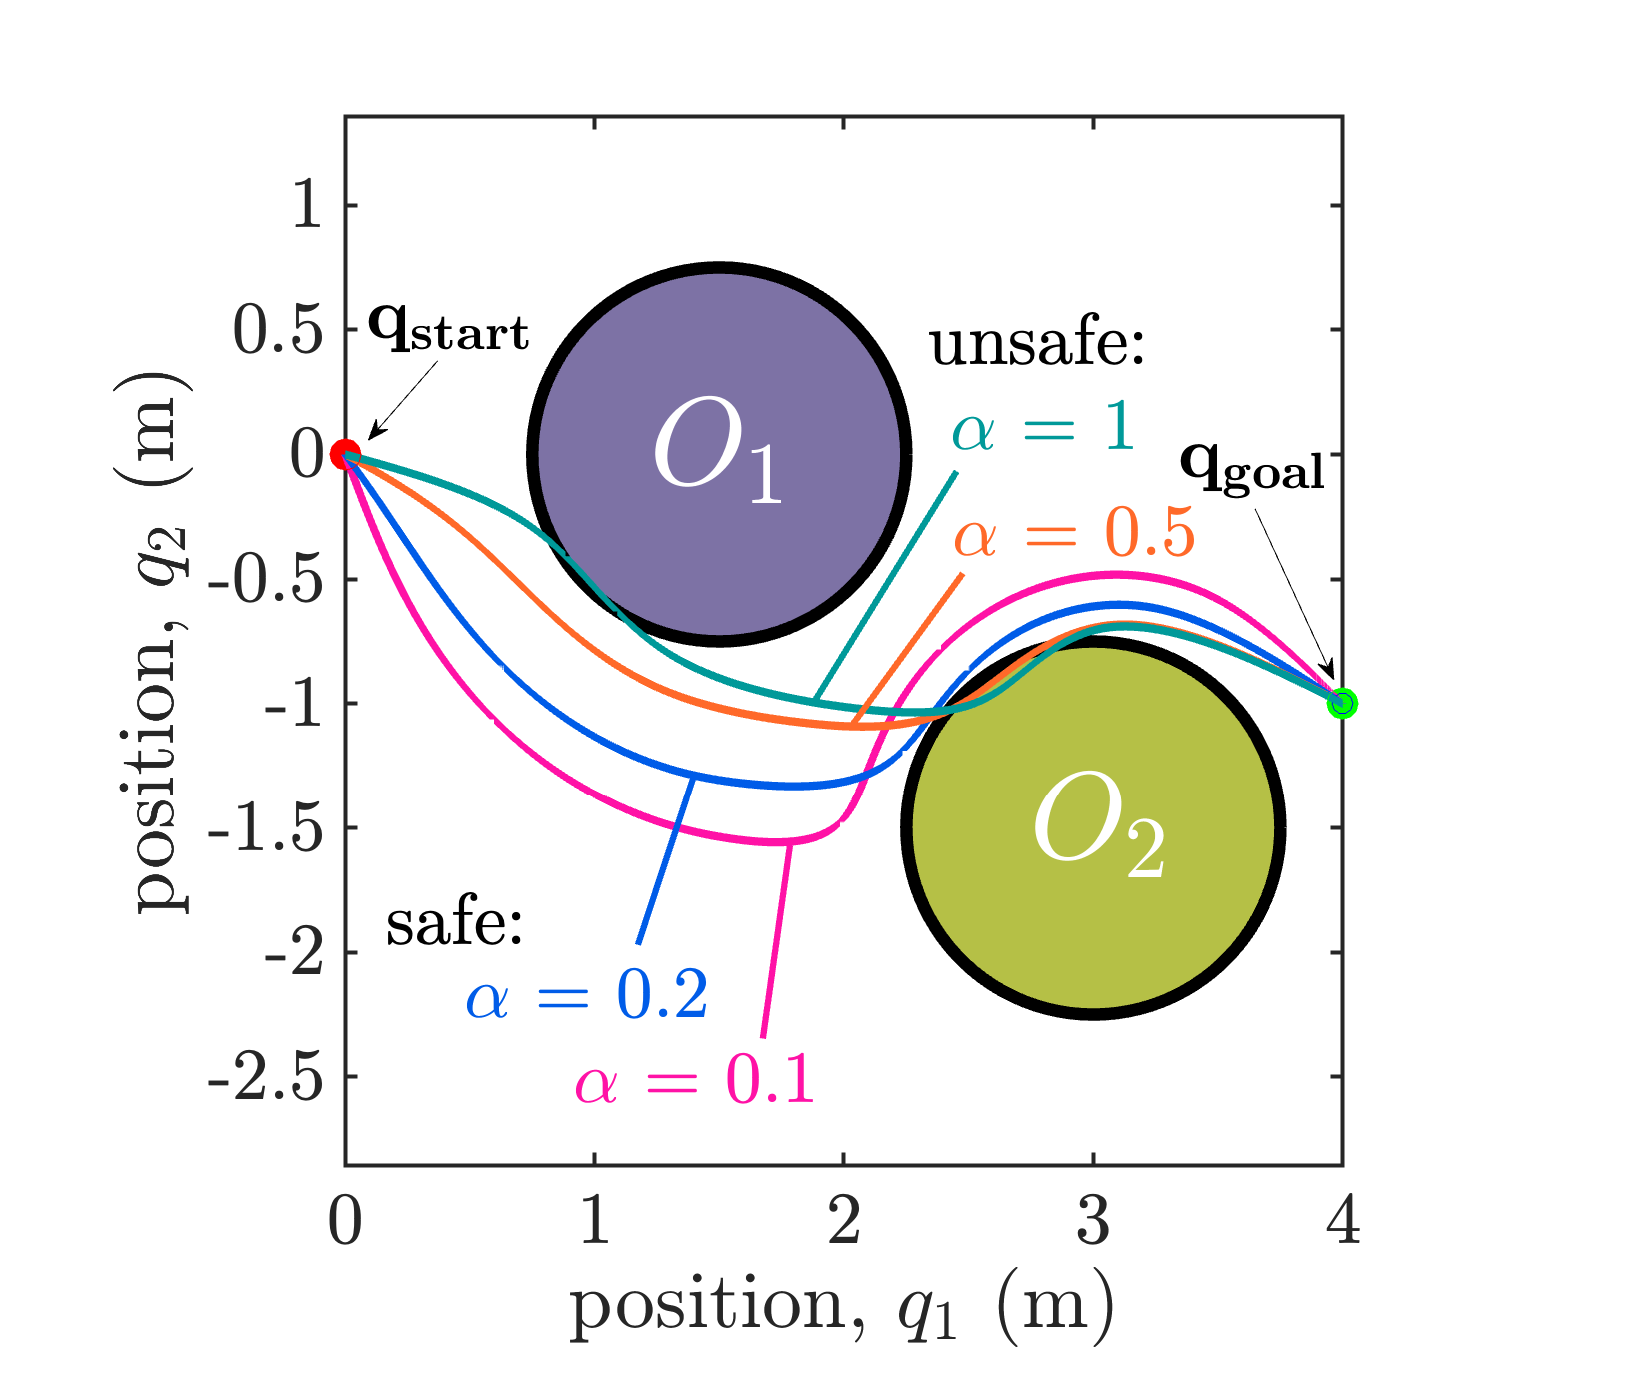
\includegraphics[scale=0.65]{figprint.eps}\\
% \subsection{Unicycle}


%%% add info on alpha ... DI, dire che stiamo utilizzando nearest obstacle
% dufferebze quando considera solo una cbf e quando di più